\addcontentsline{toc}{chapter}{Simulado 1}
\markboth{Simulado 1}{}

\num{1} Leia o trecho da notícia.

\begin{quote}
\textbf{Lei proíbe casamento a menores de 16 anos}

Você sabia que o Brasil, em números absolutos, é o quarto país onde mais
ocorrem casamentos infantis? E que 36\% das mulheres daqui se casam
antes de completarem os 18 anos? Isso é o que aponta uma pesquisa do
Banco Mundial, divulgada em 2015. Mas a perspectiva é que essa realidade
mude. Isso porque, em março de 2019, foi aprovada a Lei 13.811/19, que
proíbe o casamento para menores de 16 anos. Isso significa que agora, de
acordo com o texto, ``não será permitido, em qualquer caso, o casamento
de quem não atingiu a idade núbil'', no caso, 16 anos.

\fonte{Plenarinho. Lei proíbe casamento a menores de 16 anos. Disponível
em: https://plenarinho.leg.br/index.php/2019/03/lei-proibe-casamento-menores-de-16-anos.
Acesso em: 26 abr. 2023.}
\end{quote}

As características que dão credibilidade ao texto acima são

\begin{escolha}
\item números e dados apresentados com base em pesquisas.

\item opiniões pessoais sobre pesquisas de opinião.

\item comentários de pesquisadores e especialistas.

\item linguagem subjetiva baseada em opiniões pessoais.
\end{escolha}



\num{2} A reportagem ``Seres humanos cresceram 8,6 centímetros nos últimos cem
anos'' apresenta os resultados de um mapeamento sobre altura.

\begin{quote}
\textbf{Seres humanos cresceram 8,6 centímetros nos últimos cem anos}

Segundo uma pesquisa realizada pela revista \textit{E-Life}, os homens
mais altos do mundo são os holandeses (com uma média de 1,83 m) e as
mulheres da Letônia (1,70 m). Os mais baixinhos são do Timor Leste (1,60 m)
e as mulheres da Guatemala (1,50 m). O estudo mapeou a tendência de
crescimento em quase 200 países desde 1914.

Os pesquisadores afirmam que as mudanças nos padrões de crescimento
aconteceram, principalmente, por influências climáticas. Porém, a 
genética e as condições de saúde, saneamento e nutrição também têm sua
contribuição nestas alterações.

\fonte{Agência Brasil. Brasileiros cresceram 8,6 centímetros nos últimos cem anos.
Disponível em: www.ebc.com.br/infantil/voce-sabia/2016/07/brasileiros-cresceram-86-centimetros-nos-ultimos-cem-anos. 
Acesso em: 26 abr. 2023.}
\end{quote}

Segundo a reportagem, a média de altura dos homens do Timor Leste é

\begin{escolha}
\item menor que a das mulheres da Letônia.

\item menor que a das mulheres da Guatemala.

\item maior que a dos homens da Holanda.

\item igual à das mulheres da Letônia.
\end{escolha}


\num{3} Leia um trecho do poema ``O ramo verde'', de Adelina.

\begin{quote}
\begin{verse}
\textbf{O ramo verde}

{[}\ldots{}{]}

Foram à tarde a passeio\\
no jardim os dois; Sofia\\
colhia rosas; em meio\\
disse ao irmão: --- que alegria!

Vou dar à mamãe um \textbf{ramo}\\
das minhas amadas flores!
\end{verse}

\fonte{Adelina Lopes Vieira. Domínio Público. O ramo verde. Disponível em:
www.dominiopublico.gov.br/download/texto/wk000077.pdf.
Acesso em: 19 mar. 2023.}
\end{quote}

A palavra destacada no texto pode ser substituída, sem perda de sentido,
por:

\begin{escolha}
\item ramalhete.

\item arbusto.

\item grama.

\item espinho.
\end{escolha}

\num{4} O poema ``Dom Quixote'' mostra os irmãos Paulo e Mário unindo
forças para atingir um objetivo em comum.

\begin{quote}
\begin{verse}
\textbf{Dom Quixote}

Paulo tinha seis anos incompletos;\\
tinha só quatro o louro e gentil Mário.\\
Foram à biblioteca, sorrateiros,\\
e ficaram instantes, mudos, quietos,\\
a espreitar se alguém vinha; então, ligeiros\\
como o vento, correram para o armário,\\
que encerrava os volumes cobiçados:\\
eram dois grandes livros encarnados,\\
cheios de formosíssimas gravuras,\\
mas pesados, meu Deus!\\
Os pequeninos\\
porfiavam, cansados, vermelhitos,\\
por tirá-los da estante. Que torturas!\\
{[}...{]}\\
vamos ver à vontade o D. Quixote,\\
sem os ralhos ouvir, impertinentes,\\
da avó, que adormeceu. Oh! que ventura!
\end{verse}

\fonte{Adelina Lopes Vieira. Domínio Público. Dom Quixote. Disponível em:
www.dominiopublico.gov.br/download/texto/wk000074.pdf. 
Acesso em: 26 abr. 2023.}
\end{quote}

\begin{tabular}{ll}
\textbf{Glossário} & \mbox{}\\
cobiçados & desejados\\
porfiavam & competiam\\
ralhos & censuras\\
\end{tabular}

A intenção dos irmãos era

\begin{escolha}
\item pegar dois livros da estante sem serem vistos.

\item conseguir entrar na biblioteca sem que a avó os visse.

\item brincar na biblioteca sem que fossem vistos.

\item chamar a atenção da avó entrando na biblioteca.
\end{escolha}

\num{5} Leia o texto e responda à pergunta.

\begin{quote}
\textbf{Estado de SP realiza 'Dia V' de mobilização para aplicação de
segunda dose da vacina contra COVID-19}

\textit{Estratégia acontece no sábado (2) e também servirá para os
municípios atualizarem o sistema VaciVida e inserirem imunizados que
eventualmente ainda não foram registrados}

Governo de São Paulo anunciou nesta quarta-feira (29) o ``Dia V'' de
vacinação contra COVID-19. A iniciativa, em parceria com os 645
municípios, acontecerá neste sábado (2) e tem como objetivo a aplicação
da segunda dose da vacina e a atualização dos registros de vacinação na
plataforma VaciVida. {[}\ldots{}{]}

Mais de cinco mil pontos de vacinação no estado estarão abertos das 7h
às 19h para a aplicação exclusivamente destas doses neste sábado
(consulte a programação e horários de funcionamento dos postos de seu
município).

\fonte{Secretaria da Saúde do Estado de São Paulo. Estado de SP realiza 
Dia V de mobilização para aplicação de segunda dose da vacina contra 
COVID-19.Disponível em:
http://www.saude.sp.gov.br/ses/perfil/cidadao/homepage/destaques/estado-de-sp-realiza-dia-v-de-mobilizacao-para-aplicacao-de-segunda-dose-da-vacina-contra-covid-19.
Acesso em: 4 mai. 2023.}
\end{quote}

O texto reproduzido acima trata

\begin{escolha}
  \item do número de vacinados contra COVID-19 no estado de São Paulo.

  \item da aprovação da campanha de vacinação por parte da população.

  \item de uma mobilização para vacinação contra COVID-19.

  \item da resistência da população em tomar o imunizante.
\end{escolha}

\num{6} Leia o texto e responda à pergunta.

\begin{quote}
\textbf{Ministério da Saúde lança campanha contra malária}

\textit{Ação tem foco na Região Amazônica, com 99\% dos casos no país}

O Ministério da Saúde (MS) lançou hoje (25) uma campanha voltada para a
prevenção e combate à malária. Com o slogan \textit{O combate à malária acontece
com a participação de todos: cidadãos, comunidade e governo}, a campanha
tem como foco a Região Amazônica, que concentra 99\% dos casos no país. A
doença, cuja incidência ocorre nas populações de maior vulnerabilidade
social, representa um grande problema de saúde pública no país. A data
marca o Dia Mundial de Luta Contra a Malária e os 20 anos de atuação do
Programa Nacional de Prevenção e Controle da Malária.

\fonte{Agência Brasil. Ministério da Saúde lança campanha contra malária.
Disponível em:
https://agenciabrasil.ebc.com.br/saude/noticia/2023-04/ministerio-da-saude-lanca-campanha-contra-malaria.
Acesso em: 4 mai. 2023.}
\end{quote}

De acordo com o texto reproduzido acima, a campanha contra a Malária
terá como foco

\begin{escolha}
  \item a região Sul do Brasil

  \item ações realizadas na internet.

  \item o ensino de formas de prevenção à doença.

  \item a região amazônica.
\end{escolha}

\num{7} Leia o texto e responda à pergunta.

\begin{quote}
D. CECÍLIA (à parte) --- E titia não vem\ldots Que demora!\ldots Não sei
que lhe diga\ldots estou tão vexada\ldots (O Barão tira um livro da algibeira
e folheia-o). Se eu pudesse deixá-lo\ldots É o que vou fazer. (Sobe).

BARÃO (fechando o livro e erguendo-se) --- V. Excia. há de desculpar-me.
Recebi hoje mesmo este livro da Europa; é obra que vai fazer revolução na
ciência; nada menos que uma monografia das gramíneas, premiadas pela 
Academia de Estocolmo.

\fonte{Machado de Assis. Lição de Botânica. Disponível em:
<https://machado.mec.gov.br/obra-completa-lista/item/download/65\_2b8fb9ad43aa37653a58bc2bd56e33aa>.
Acesso em: 23 abr. 2023.}
\end{quote}

Tendo em vista as características formais do gênero dramático, quais são
as personagens envolvidas no trecho transcrito acima?

\begin{multicols}{2}
\begin{escolha}

  \item D. Cecília e Barão.

  \item Machado de Assis e D. Cecília.

  \item Barão.

  \item D. Cecília.

\end{escolha} 
\end{multicols}


\num{8} Leia o texto e responda à pergunta.

\begin{quote}
\begin{verse}
\textbf{O mar}

Que nostalgia vem de tuas vagas\\
Ó velho mar, ó lutador Oceano!\\
Tu de saudades íntimas alagas\\
O mais profundo coração humano.

Sim! Do teu choro enorme e soberano,\\
Do teu gemer nas desoladas plagas\\
Sai o que quer que é, rude sultão ufano,\\
Que abre nos peitos verdadeiras chagas.

Ó mar! Ó mar! Embora esse eletrismo,\\
Tu tens em ti o germe do lirismo.\\
És um poeta lírico demais.

E eu para rir com humor das tuas\\
Nevroses colossais, bastam-me as luas\\
Quando fazem luzir os seus metais.
\end{verse}

\fonte{Cruz e Sousa. O Mar. Disponível em:
https://pt.wikisource.org/wiki/O\_Mar\_(Cruz\_e\_Sousa). Acesso em 4 mai. 2023.}
\end{quote}

O texto acima está organizado em versos e estrofes; logo, trata-se de
um

\begin{escolha}
  \item poema.

  \item romance.

  \item anúncio.

  \item drama.
\end{escolha}

\pagebreak
\num{9} Leia o texto e responda à pergunta.

\begin{quote}
--- Vou ser atacado? exclamou D. Antônio pensativo.

--- Sim: podes contar.

--- \textbf{E por quem?}

--- Pelo Aimoré.

--- \textbf{E como sabes isto?} --- perguntou D. Antônio fitando nele um olhar
desconfiado.

\fonte{José de Alencar. O Guarani. Disponível em:
<https://pt.wikisource.org/wiki/O\_Guarani/II/X>. Acesso em: 4 mai.
2023.}
\end{quote}

O sinal de pontuação utilizado nos trechos destacados indica

\begin{escolha}
  \item o final de uma frase.

  \item uma frase destacada.

  \item uma dúvida.

  \item a divisão de uma frase.
\end{escolha} 


\pagebreak
\num{10} Observe a imagem e responda à pergunta.

\begin{figure}[htpb!]
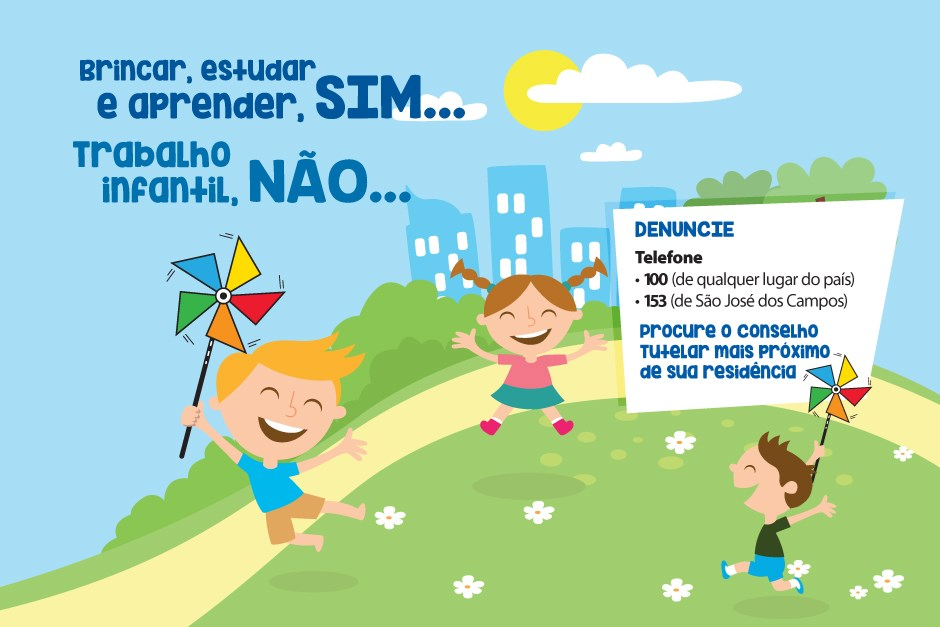
\includegraphics[width=\textwidth]{./imgQ4PORT/media/image1.jpeg}
\caption{A Prefeitura de São José dos Campos realiza durante todo o mês
de junho, uma série de ações para alertar a população sobre o
crescimento do trabalho infantil}
\end{figure}

\fonte{Prefeitura de São José dos Campos. São José realiza campanha contra
o trabalho infantil. Disponível em: <https://www.sjc.sp.gov.br/noticias/2021/maio/31/sao-jose-realiza-campanha-contra-o-trabalho-infantil/>.
Acesso em: 4 mai. 2023.}

Na imagem acima, um recurso utilizado para convencer o público é/são

\begin{escolha}
  \item as figuras coloridas.

  \item o uso das palavras ``sim'' e ``não'' em letras maiúsculas.

  \item os semblantes tristes das crianças.

  \item o uso da linguagem formal.
\end{escolha}

\pagebreak
\num{11} Leia o texto e responda à pergunta.

\begin{quote}
--- Como vai, bacharel?

--- Menos mal, ignoto viajor.

--- Tomando a fresca, não?

--- \textit{C'est vrai}, como dizem os franceses.

--- Bem, té-logo bacharel, estou meio afobado\...

\fonte{Mário de Andrade. Macunaíma. Disponível em:
<https://pt.wikisource.org/wiki/Macunaíma/1928/IV>. Acesso em: 4
mai. 2023.}
\end{quote}

No texto reproduzido acima, encontramos o uso de uma variante informal
da língua portuguesa na expressão

\begin{multicols}{2}
\begin{escolha}
  \item ignoto viajor 

  \item \textit{C'est vrai}

  \item té logo

  \item Como vai, bacharel?
\end{escolha}
\end{multicols}

\num{12} Leia o texto e responda à pergunta.

\begin{quote}
\textbf{Bullying: combate deve ser feito de forma coletiva e intersetorial}

Um em cada três alunos em todo o mundo já foi vítima de
\textit{bullying},segundo a Organização das Nações Unidas para Educação,
Ciência e Cultura (Unesco). Esse tipo de violência, ainda comum nas
escolas, \textbf{gera consequências arrasadoras no desempenho dos alunos},
além de sequelas negativas para a saúde física e mental das crianças.
Hoje (7) é comemorado no país o Dia Nacional de Combate ao Bullying e à
Violência nas Escolas.

\fonte{Agência Brasil. Bullying: combate deve ser feito de forma coletiva
e intersetorial. 
Disponível em: https://agenciabrasil.ebc.com.br/educacao/noticia/2023-04/bullying-combate-deve-ser-feito-de-forma-coletiva-e-intersetorial. 
Acesso em: 4 mai. 2023.}
\end{quote}

\pagebreak
O adjetivo encontrado no trecho destacado indica uma conotação

\begin{escolha}
  \item negativa.

  \item positiva.

  \item indiferente.

  \item duvidosa.
\end{escolha}


\num{13} Leia o texto e responda à pergunta.

\begin{quote}
\textbf{No verão, banhistas devem redobrar os cuidados para evitar
afogamentos}

Tempo quente e férias. Essa é a combinação ideal para que praias e
piscinas fiquem repletas de banhistas. Mas alguns cuidados são
fundamentais para que diversão não coloque a vida das pessoas em risco.
Segundo dados do Corpo de Bombeiros, no ano passado foram registrados
3,1 mil afogamentos no Estado, um aumento de 11,7\% em relação a 2021,
quando ocorreram 2,81 mil casos em SP.

``Neste verão, não abuse da sorte e, na praia, sempre respeite as
orientações do salva-vidas. Lembre-se de que quase metade dos afogados
acreditavam que sabiam nadar'', alerta a coordenadora do Grupo de
Atendimento e Resgate às Urgências (Grau), Cecilia Damasceno.

\fonte{Secretaria da Saúde do Estado de São Paulo. No verão, banhistas 
devem redobrar os cuidados para evitar afogamentos. Disponível em:
http://www.saude.sp.gov.br/ses/perfil/cidadao/homepage/destaques/no-verao-banhistas-devem-redobrar-os-cuidados-para-evitar-afogamentos>.
Acesso em 4 mai. 2023.}
\end{quote}

A citação de uma especialista no assunto tratado no texto torna o
argumento mais

\begin{multicols}{2}
\begin{escolha}
  \item confuso.

  \item restrito.

  \item subjetivo.

  \item confiável.
\end{escolha}
\end{multicols}

\pagebreak

\num{14} Observe a imagem e responda à pergunta.

\begin{figure}[htpb!]
\centering
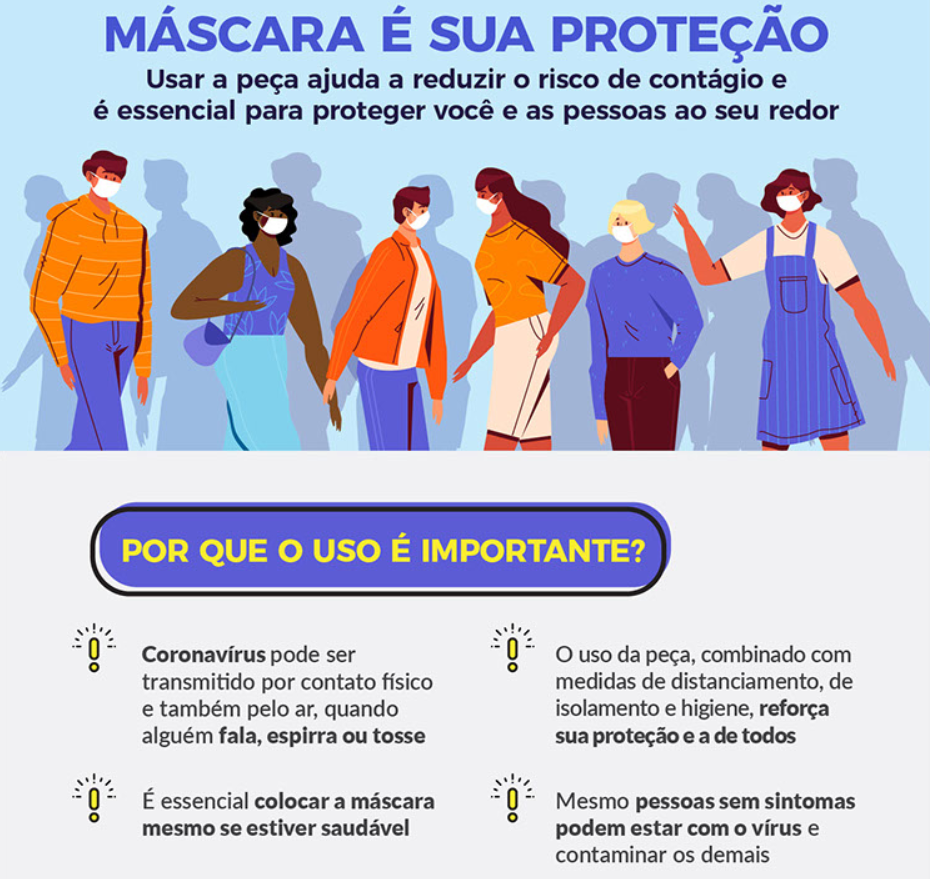
\includegraphics[width=.9\textwidth]{./imgQ4PORT/media/image2.png}
\end{figure}

\fonte{Governo do Estado de São Paulo. Entenda por que uso da máscara
ajuda a reduzir risco de contaminação por COVID-19.Disponível em:
<https://www.saopaulo.sp.gov.br/spnoticias/entenda-por-que-uso-da-mascara-ajuda-a-reduzir-risco-de-contaminacao-por-covid-19/>.
Acesso em: 4 mai. 2023.}

De acordo com o infográfico, a máscara de proteção

\begin{escolha}
  \item ajuda a evitar a transmissão do vírus pelo ar.

  \item não deve ser usada por crianças.

  \item protege apenas seu usuário.

  \item deverá ser utilizada somente se o indivíduo estiver doente.
\end{escolha}


\num{15} Leia o texto e responda à pergunta.

\begin{quote}
\textbf{``Não sou o substituto do Google'', afirma ChatGPT ao ser entrevistado}

Desde que foi apresentado ao mundo, em novembro de 2022, ainda em uma
versão de teste, o ChatGPT vem causando assombro. A reação inicial de
quem vê o sistema de inteligência artificial (criado pela empresa
norte-americana OpenAI em funcionamento) respondendo a uma pergunta
qualquer, pode variar entre o fascínio e o entusiasmo. Em um segundo
momento, contudo, é inevitável pensar nas consequências de tamanho salto
tecnológico. {[}\ldots{}{]}

Por ora, o ChatGPT produz apenas textos sobre praticamente qualquer
assunto, no formato requisitado pelo usuário. Há, no entanto, outros
programas de inteligência artificial capazes de gerar imagens
\textbf{hiper-realistas} a partir de descrições textuais fornecidas pelos
usuários.

\fonte{Agência Brasil. Não sou o substituto do Google, afirma ChatGPT ao
ser entrevistado. Disponível em: https://agenciabrasil.ebc.com.br/geral/noticia/2023-01/nao-sou-o-substituto-do-google-afirma-chatgpt-ao-ser-entrevistado. com alterações. 
Acesso em: 4 mai. 2023}
\end{quote}

O prefixo ``hiper'' destacado no trecho acima indica

\begin{escolha}
  \item negação.

  \item intensidade.

  \item diminuição.

  \item oposição.
\end{escolha}


\vspace*{-3.4cm}
\hspace*{-3.7cm}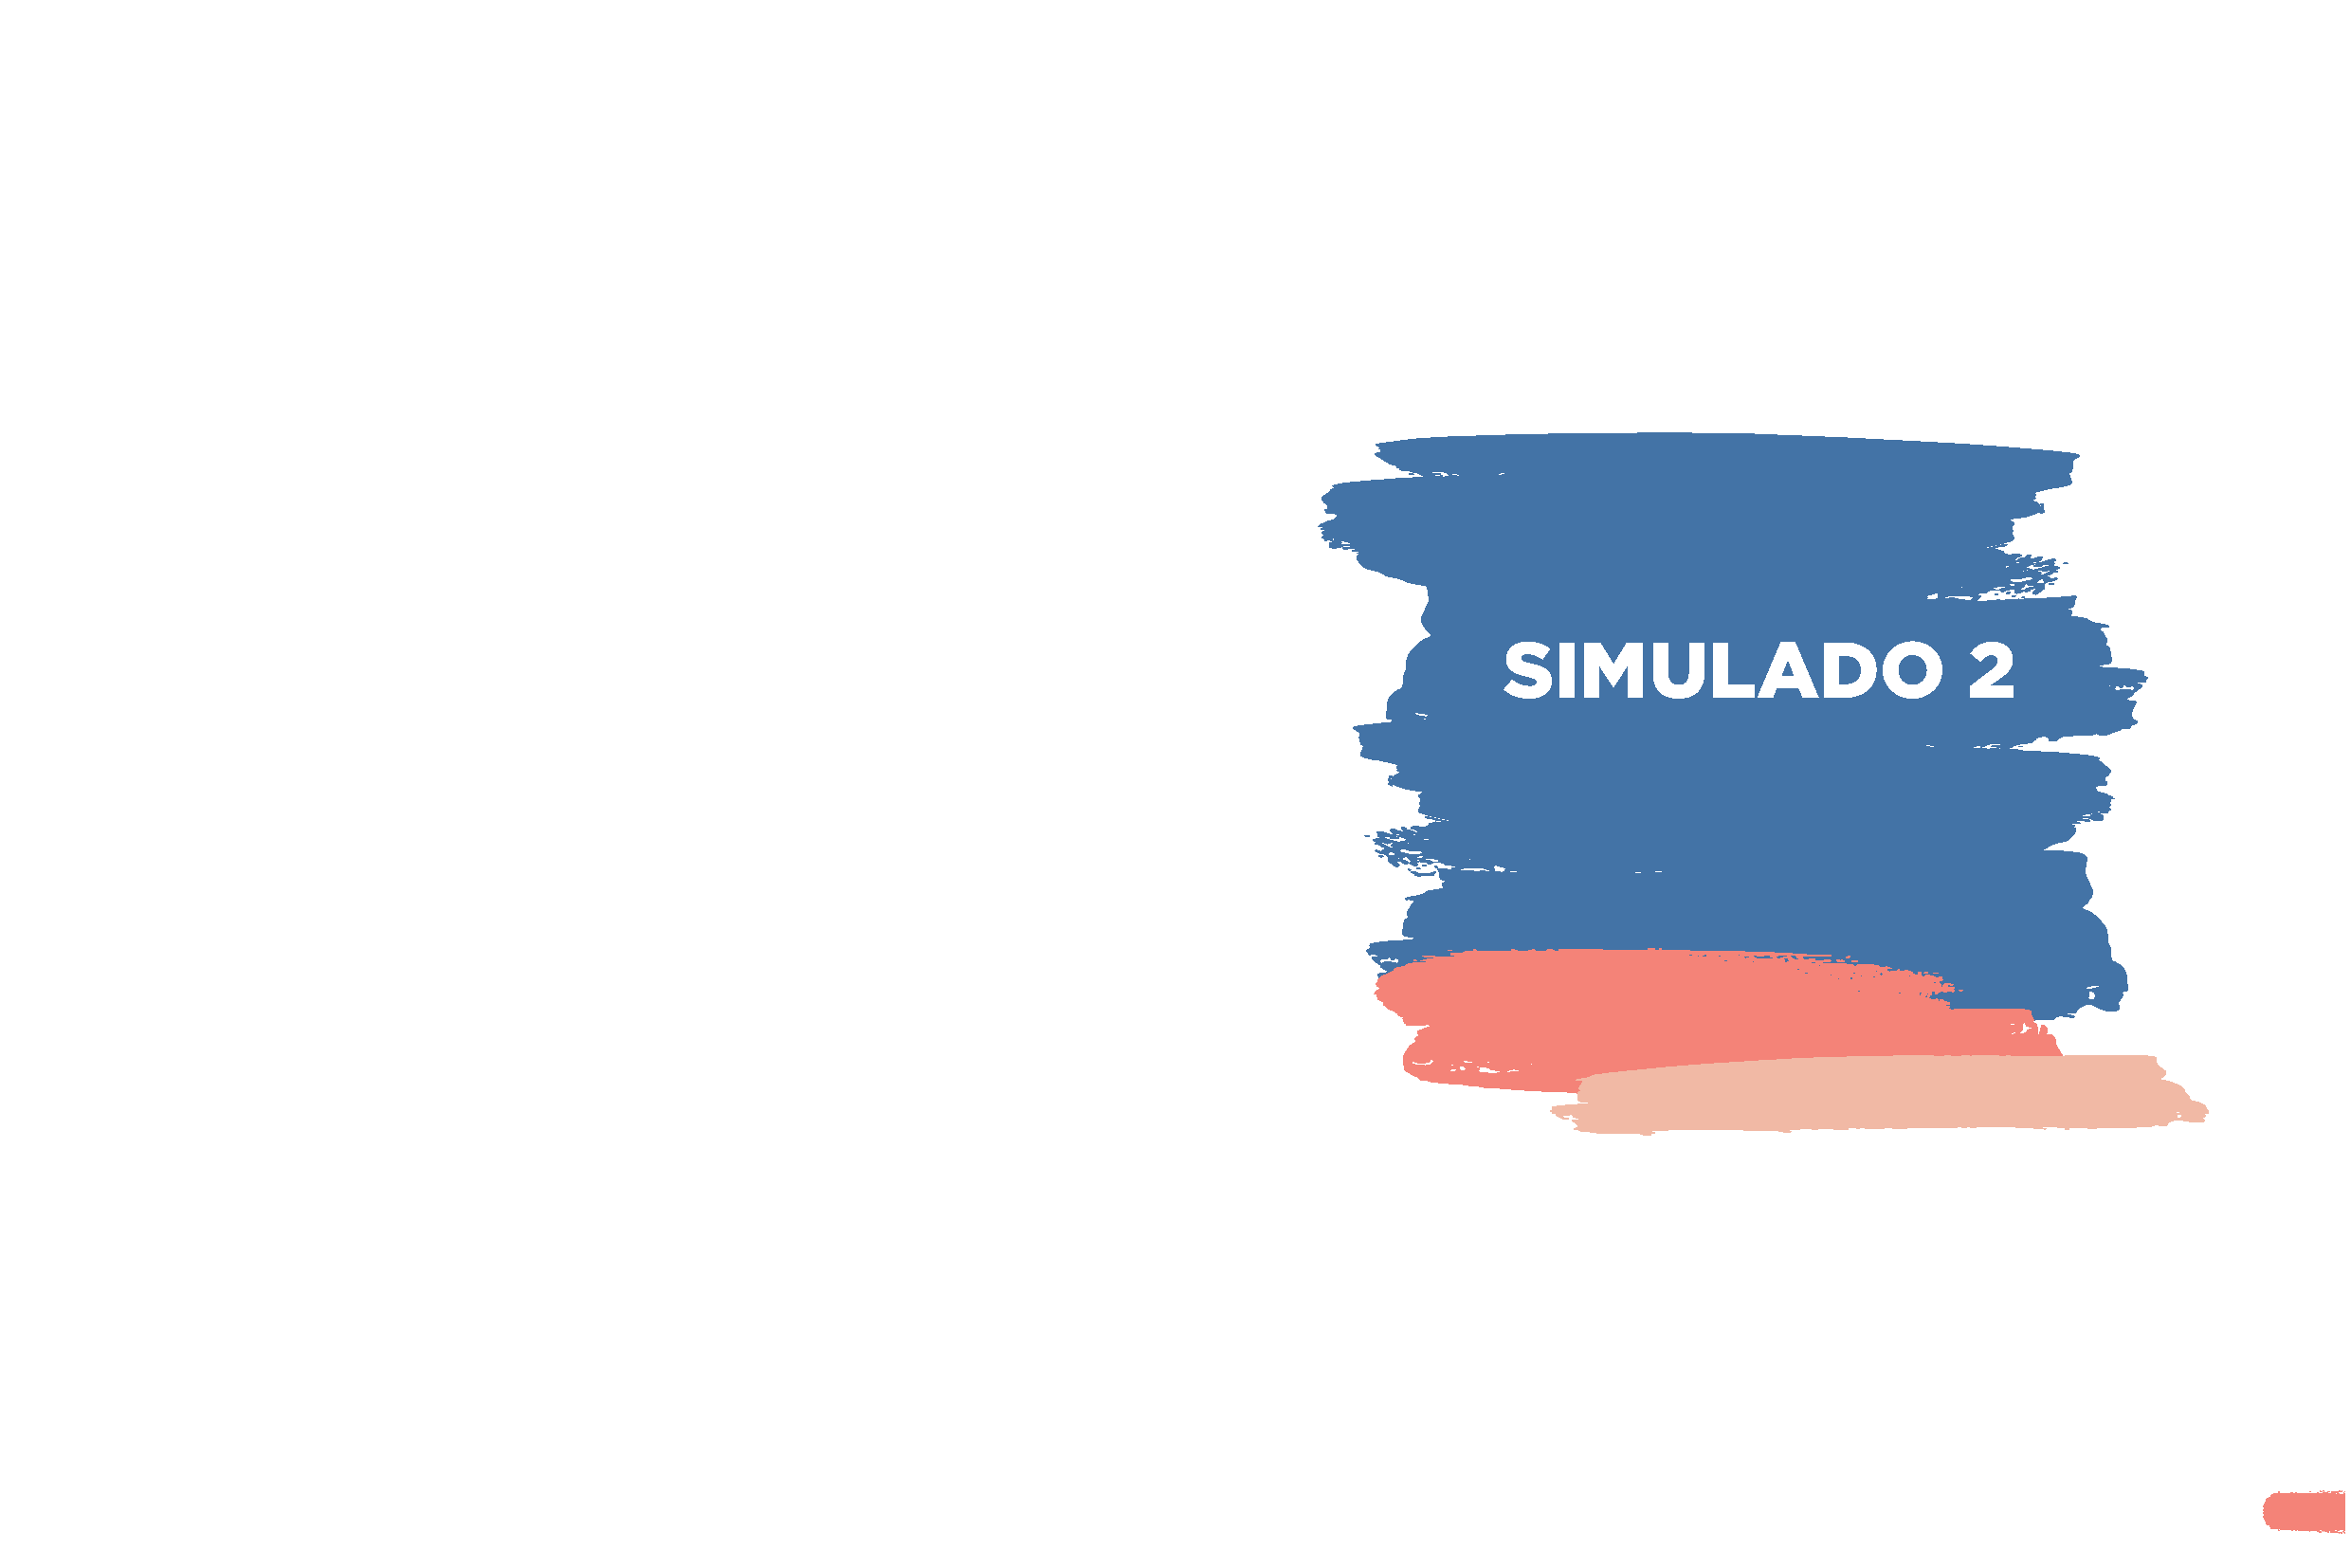
\includegraphics[scale=1]{../watermarks/2simulado5ano.pdf}
\addcontentsline{toc}{chapter}{Simulado 2}
\markboth{Simulado 2}{}

\num{1} Leia a fábula para responder à questão.

\begin{quote}
\textbf{Os viajantes e o urso}

Dois homens viajavam juntos quando, de repente, surgiu um urso de dentro
da floresta e parou diante deles, urrando. um dos homens tratou de subir
na árvore mais próxima e agarrar-se aos ramos. O outro, vendo que não
tinha tempo para esconder-se, deitou-se no chão, esticado, fingindo de
morto {[}\ldots{}{]}.

\textbf{Na hora do perigo é que se conhece os amigos.}

\fonte{Ana Rosa Abreu e outros autores. Os viajantes e o urso.
Alfabetização, Vol.2: contos, fábula, lendas e mitos. Disponível em:
www.dominiopublico.gov.br/download/texto/me000589.pdf.
Acesso em: 24 abr. 2023.}
\end{quote}

Na leitura da fábula, pode-se compreender que o homem que subiu na árvore

\begin{escolha}
\item abandonou o amigo no perigo, em vez de ajudá-lo.

\item pensou rápido em como ele e seu amigo podiam se proteger.

\item ajudou seu amigo, pois mostrou uma forma de se esconder.

\item aconselhou o amigo a se fingir de morto para se esconder.
\end{escolha}


\enlargethispage{\baselineskip}
\num{2} Leia o trecho de uma carta do leitor coletiva.

\begin{quote}
Olá, CHC! Somo alunos do 5º ano. Lemos durante toda a semana na nossa
roda de leitura curiosidades e histórias da revista CHC. Lemos o texto
``Por que o cérebro nunca deixa de aprender?'' e achamos muito legal.
Gostamos da parte que fala que o cérebro de uma criança armazena
informações muito mais rapidamente que o de um adulto. Por isso, vamos
continuar lendo as matérias publicadas na revista. Assim vamos aprender
muito mais, não acha?

\begin{flushleft}
\textit{Alunos do 5º ano D. Escola Estadual José Ariano Rodrigues. Lins/SP.}
\end{flushleft}

%\fonte{Ciência Hoje das Crianças. Neurônios em movimento. Disponível em: http://chc.org.br/artigo/fala-aqui/. Acesso em: 26 abr. 2023.}
\end{quote}

Pela leitura da carta do leitor, entende-se que o seu tema central é

\begin{escolha}
\item os elogios dos alunos à revista e ao texto ``Por que o cérebro nunca 
deixa de aprender?''.

\item a pergunta para a revista se eles concordam que ler mais permite que
se aprenda mais também.

\item a roda de leitura que as crianças fazem na escola para discutir
os textos da revista.

\item a frequência com que as crianças leem a revista, sendo que, por
isso, elas aprenderão muito mais.
\end{escolha}



\num{3} Leia um trecho do conto tradicional ``João e Maria'', duas crianças muito pobres.

\begin{quote}
\textbf{João e Maria}

Às margens de uma extensa mata existia, há muito tempo, uma cabana
pobre, feita de troncos de árvore, na qual morava um lenhador com sua
segunda esposa e seus dois filhinhos, nascidos do primeiro casamento. 
O garoto chamava-se João e a menina, Maria.

\fonte{Ana Rosa Abreu e outros autores. João e Maria.
Alfabetização, Vol.2: contos, fábula, lendas e mitos. Disponível em:
www.dominiopublico.gov.br/download/texto/me000589.pdf.
Acesso em: 26 abr. 2023.}
\end{quote}

No trecho, os artigos

\begin{escolha}
\item ``um'' e ``uma'' são utilizados para se referir a seres que não estão vivos.

\item ``o'' e ``a'' são utilizados para se referir às personagens principais.

\item femininos são utilizados para se referir a seres que não estão vivos.

\item masculinos são utilizados para todas as personagens da história.
\end{escolha}

\pagebreak
\num{4} Quando não se sabe o significado de uma palavra, muitas vezes, é
possível inferi-lo a partir da análise do contexto em que ela está
inserida.

\begin{quote}
\textbf{Dos 4 aos 6 anos, crianças têm um salto de desenvolvimento em autonomia}

Quando completam 4 anos de idade, as crianças já percorreram um amplo
caminho de desenvolvimento. Estão já bastante independentes e conseguem
fazer algumas atividades simples da rotina praticamente sem ajuda, como
escovar os dentes, escolher as roupas e se vestir. Nessa etapa, é muito
importante incentivar essas conquistas e apoiar sua crescente autonomia.
{[}...{]}

Ao longo dessa etapa, também haverá muitos ganhos \textbf{cognitivos}. A
capacidade de raciocínio aumenta e possibilita que a criança faça
relações mais complexas. Com 6 anos, muitas já conseguem levar em
consideração regras de diferentes situações sociais e diferenciar com
clareza acontecimentos reais daqueles que são faz-de-conta.

\fonte{Agência Brasil. Dos 4 aos 6 anos, crianças têm um salto de desenvolvimento em autonomia. 
Disponível em:
www.ebc.com.br/infantil/para-pais/2016/10/dos-4-aos-6-anos-criancas-tem-um-salto-de-desenvolvimento-em-autonomia.
Acesso em: 19 mar. 2023.}
\end{quote}

Analisando a palavra destacada no contexto em que se insere, 
pode-se afirmar que diz respeito

\begin{escolha}
\item ao ganho de conhecimento.

\item ao desenvolvimento da fala.

\item aos movimentos corporais.

\item às regras de convívio.
\end{escolha}

\pagebreak
\num{5} Leia o texto e responda à pergunta.

\begin{quote}
Já se não ria; tinha só um resto de sorriso forçado e resignado. Olhou
bem para ela, e perguntou-lhe o que era.

--- Você promete o que lhe disse?

--- Vá lá. Que foi?

--- Pois saiba que ouvi nada menos que uma declaração de amor.

\fonte{Machado de Assis. Quincas Borba. Disponível em:
https://machado.mec.gov.br/obra-completa-lista/item/download/14\_7bbc6c42393beeac1fd963c16d935f40.
Acesso em: 4 mai. 2023.}
\end{quote}

Os travessões empregados no trecho acima cumprem a função de

\begin{escolha}
  \item descrever a aparência das personagens.

  \item introduzir a fala de uma personagem.

  \item concluir um parágrafo da narrativa.

  \item introduzir a descrição do espaço.
\end{escolha}

\num{6} Leia o texto e responda à pergunta.

\begin{quote}
Que tal agora desenhar a sua própria amarelinha? Para facilitar, siga o
passo a passo:

1. Você vai precisar de giz e uma pedrinha;

2. Desenhe a sequência de números de 1 a 10 (quadrados) no chão;

3. Vamos às regras: Ninguém pode pisar fora do quadrado; a pedrinha
precisa ficar dentro da marcação e do número correto; só pode colocar um
pé em cada quadrado; quando for um quadrado, pule de um pé só e, quando
tiver dois, é um pé em cada; não pode pisar no quadrado que estiver com a
pedra; deve recolher a pedra na volta.

4. Se possível convide sua família ou amigos para brincar com você.

\fonte{Secretaria Municipal de Educação de Goiânia. Brincar de 
Amarelinha. Disponível em:
https://sme.goiania.go.gov.br/conexaoescola/ensino\_fundamental/brincar-de-amarelinha/.
Acesso em: 4 mai. 2023.}
\end{quote}

As instruções para a brincadeira descrita no texto acima são
introduzidas por

\begin{multicols}{2}
\begin{escolha}
  \item verbos no imperativo.

  \item verbos no indicativo.

  \item adjetivos.

  \item substantivos.
\end{escolha}
\end{multicols}


\num{7} Leia o texto e responda a pergunta.

\begin{quote}
\textbf{O velho abriu as pálpebras e cerrou-as logo:}

--- Filha de Araken, escolhe para teu hóspede o presente da volta e
prepara o moquém da viagem. Se o estrangeiro precisa de guia, o
guerreiro Cauby, senhor do caminho, o acompanhará.

\fonte{José de Alencar. Iracema. Disponível em:
https://pt.wikisource.org/wiki/Iracema. Acesso em: 4 mai. 2023. com
adaptações.}
\end{quote}

O sinal de pontuação utilizado no final do trecho destacado cumpre a
função de

\begin{escolha}
  \item concluir uma frase.

  \item enfatizar um dos termos da frase.

  \item marcar uma dúvida da personagem.

  \item indicar o início de um diálogo.
\end{escolha}

\pagebreak
\num{8} Leia o texto e responda à pergunta.

\begin{quote}
\textbf{Formação de professores é entrave ao uso de tecnologia em sala de
aula}

Estudo do British Council --- organização internacional do Reino Unido
para relações culturais e oportunidades educacionais --- mostra que a
formação docente é um dos mais graves empecilhos ao uso de tecnologia em
laboratórios ou em sala de aula. Paralelamente a essa questão, as
escolas brasileiras enfrentam problemas de infraestrutura.

Os dados constam do estudo \textit{O ensino de ciências da natureza e suas
tecnologias na educação básica brasileira -- um panorama entre os anos
de 2010 e 2020}, feito em parceria com a Fundação Carlos Chagas e lançado
nesta quarta-feira (12).

\fonte{Agência Brasil. Formação de professores é entrave ao uso de
tecnologia em sala de aula. Disponível em:
https://agenciabrasil.ebc.com.br/educacao/noticia/2023-04/formacao-de-professores-e-entrave-ao-uso-de-tecnologia-em-sala-de-aula.
Acesso em: 4 mai. 2023.}
\end{quote}

Após a leitura do texto, pode-se inferir que

\begin{escolha}
  \item o uso da tecnologia é muito importante no contexto da sala de aula.

  \item o uso da tecnologia deve ser evitado no contexto da sala de aula.

  \item os professores brasileiros sabem utilizar tecnologia em sala de aula.

  \item as escolas brasileiras utilizarão tecnologias britânicas em sala de
aula.
\end{escolha}



\num{9} Leia o texto e responda à pergunta.

\begin{quote}
Si fosse ser água os outros bebiam, si fosse ser formiga esmagavam, si
fosse mosquito flitavam, si fosse trem de ferro descarrilava, si fosse
rio punham no mapa \ldots Resolveu:

``Vou ser Lua''. Gritou:

--- Abram a porta, gente, que quero umas coisas!

\fonte{Mário de Andrade. Macunaíma. Disponível em:
https://pt.wikisource.org/wiki/Macunaíma/1928. Acesso em: 4 mai.
2023.}
\end{quote}

No trecho reproduzido acima, o verbo utilizado para introduzir uma fala
é

\begin{escolha}
  \item ``abram''.

  \item ``gritou''.

  \item ``punham''.

  \item ``fosse''.
\end{escolha}

\num{10} Leio texto e responda à pergunta.

\begin{quote}
Se, em conversa com o ex-presidente de província, disse todo o bem que
pensava do Governo Provisório, não lhe ouviu palavras de acordo nem de
contestação. Não entrou mais fundo na confissão do homem, porque a moça
o atraía, e ele gostava mais \textbf{dela} que do pai.

\fonte{Machado de Assis. Esaú e Jacó. Disponível em:
https://machado.mec.gov.br/obra-completa-lista/item/download/12\_ab2c739d2e8293712078e7b6b0c12abb.
Acesso em: 4 mai. 2023.}
\end{quote}

O termo destacado no trecho acima é utilizado para retomar a palavra

\begin{escolha}
  \item ``confissão''.

  \item ``palavras''.

  \item ``moça''.

  \item ``ele''.
\end{escolha}

\pagebreak
\num{11} Leia o texto e responda à pergunta.

\begin{quote}
\textbf{Brasileiros preferem cursos online para qualificação profissional}

Cursos online têm uma vantagem em termos de se adequar mais ao tempo das
pessoas, embora um curso presencial, a interação com os colegas e
professores ao vivo, tenha as suas vantagens. ``Eu diria que um curso
híbrido \textbf{talvez} seja uma solução a esses cursos puramente digitais,
embora reconheça que sejam mais complexos e caros esses cursos que têm
um lado presencial'', afirmou o diretor da FGV Social.

\fonte{Agência Brasil. Brasileiros preferem cursos online para
qualificação profissional. Disponível em:
https://agenciabrasil.ebc.com.br/geral/noticia/2023-04/brasileiro-prefere-cursos-online-para-qualificacao-ao-mercado.
Acesso em: 25 abr. 2023.}
\end{quote}

O termo destacado no trecho acima indica

\begin{escolha}
  \item lugar.

  \item tempo.

  \item negação.

  \item dúvida.
\end{escolha}



\num{12} Leia o texto e responda à pergunta.

\begin{quote}
\textbf{Centro de Referência em Saúde Indígena é inaugurado em terra
Yanomami}

O território Yanomami em Surucucu recebeu um Centro de Referência em
Saúde Indígena para combater crise humanitária de saúde no local. A
unidade foi inaugurada nessa sexta-feira (21) e é preparada para
atendimentos de urgência, consultas, exames e o tratamento de malária e
desnutrição. Desde o começo do ano, o governo federal mobiliza uma
operação interministerial para o atendimento aos povos dessa região.

\fonte{Agência Brasil. Centro de Referência em Saúde Indígena é inaugurado
em terra Yanomami. Disponível em: https://agenciabrasil.ebc.com.br/saude/noticia/2023-04/centro-de-referencia-em-saude-indigena-e-inaugurado-em-terra-yanomami. Acesso em: 4 mai. 2023}
\end{quote}

O texto acima cumpre a função de informar o leitor a respeito de um
acontecimento; logo, trata-se de um(a)

\begin{escolha}
  \item anúncio.

  \item poema.

  \item notícia.

  \item conto.
\end{escolha}



\num{13} Leia o texto e responda à pergunta.

\begin{quote}
\textbf{Governo de SP amplia Campanha de Multivacinação até 30 de novembro}

Devido à baixa procura, o Governo de SP amplia a Campanha de
Multivacinação e até o final de novembro, quando crianças e adolescentes
com menos de 15 anos podem atualizar a caderneta de vacinação. Apenas
34\% do público-alvo, entre crianças e adolescentes de até 15 anos de
idade, procuraram os postos para se vacinar.

``É imprescindível que pais e responsáveis levem seus filhos aos postos
para tomarem os imunizantes e, deste modo, garantirem a saúde e
segurança de suas famílias e da sociedade. As baixas procuras estão
ameaçando o retorno de doenças já erradicadas, é preciso aproveitar a
oportunidade para prevenir e salvar'', destaca Tatiana Lang, do Centro de
Vigilância Epidemiológica da Secretaria de Estado da Saúde.

\fonte{Governo de São Paulo. Governo de SP amplia Campanha de
Multivacinação até 30 de novembro. Disponível em:
https://www.saopaulo.sp.gov.br/spnoticias/governo-de-sp-amplia-campanha-de-multivacinacao-ate-30-de-novembro/.
Acesso em: 24 abr. 2023.}
\end{quote}

O texto reproduzido acima pode ser considerado mais eficiente por
apresentar

\begin{escolha}
  \item perspectivas conflitantes.

  \item a opinião de uma especialista.

  \item uma linguagem complexa.

  \item informações confusas.
\end{escolha}



\num{14} Leia o texto e responda à pergunta.

\begin{quote}
\begin{verse}
\textbf{O muro}

Movendo os pés doirados, lentamente,\\
Horas brancas lá vão, de amor e rosas\\
As impalpáveis formas, no ar, cheirosas\\
Sombras, sombras que são da alma doente!
\end{verse}

\fonte{Pedro Kilkerry. O Muro. Disponível em:
https://pt.wikisource.org/wiki/O\_Muro.
Acesso em 4 mai. 2023.}
\end{quote}

A rima entre as palavras ``rosas'' e ``cheirosas'' encontrada na primeira
estrofe indica uma relação de

\begin{escolha}
  \item oposição.

  \item aproximação.

  \item contraste.

  \item negação.
\end{escolha}

\num{15} Observe a imagem e responda à pergunta.

\begin{quote}
\begin{wrapfigure}{r}{.5\textwidth}
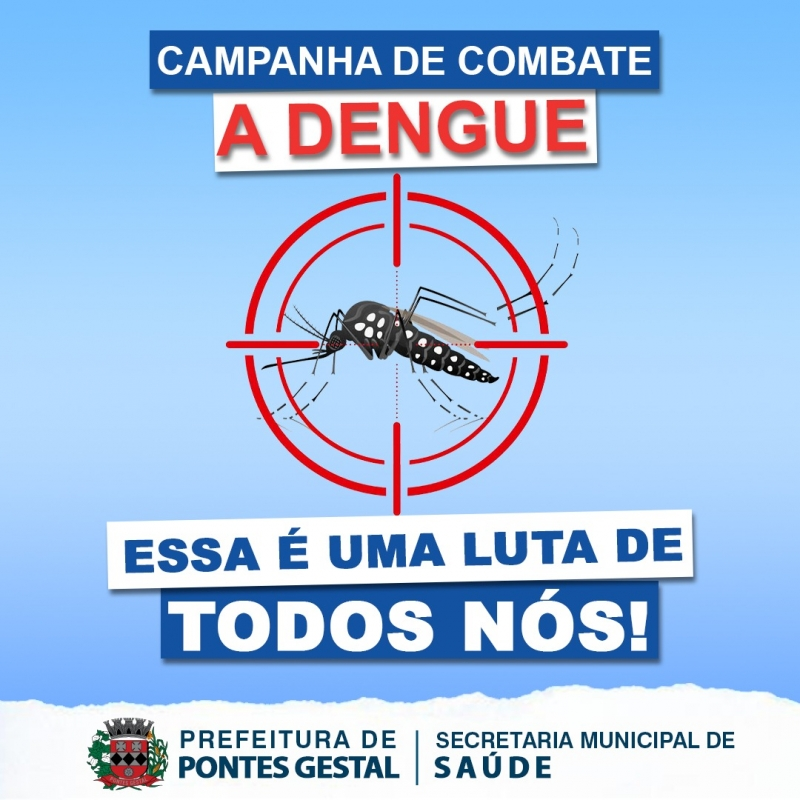
\includegraphics[width=.5\textwidth]{./imgQ4PORT/media/image3.jpeg}
%\caption{Foto Noticia Principal Grande}
\end{wrapfigure}

O calor e as chuvas constantes são alguns dos fatores que mais
favorecem a proliferação do \textit{Aedes aegypti}, mosquito transmissor da
dengue, zika e chikungunya. Por isso, o número de casos dessas doenças
vem aumentando a cada dia. Grande parte dos focos estão dentro das
residências e para evitar que o mosquito se prolifere, simples atitudes
como virar para baixo garrafas, colocar telas nas janelas, deixar sempre
com areia os pratos de plantas, manter calhas e vasilhas de animais de
estimação sempre limpas, fazem a diferença no combate do mosquito 
\textit{Aedes aegypti}. Vale ressaltar que o descarte incorreto de 
lixo é uma das principais causas para o acúmulo de larvas dos mosquitos,
por isso, descarte seu lixo no local adequado. Todos juntos contra a
Dengue! Já combateu o mosquito hoje? Faça a sua parte e ajude a mantê-lo
longe em 2022!

\fonte{Prefeitura Municipal de Pontes Gestal. Campanha conta dengue.
Disponível em: https://www.pontesgestal.sp.gov.br/portal/noticias/0/3/435/campanha-contra-a-dengue.
Acesso em: 4 mai. 2023}
\end{quote}

A ilustração reproduzida acima estabelece com o texto uma relação de

\begin{multicols}{2}
\begin{escolha}

  \item contraste.

  \item repetição.

  \item complementação.

  \item negação.

\end{escolha}
\end{multicols}

\vspace*{-3.4cm}
\hspace*{-3.7cm}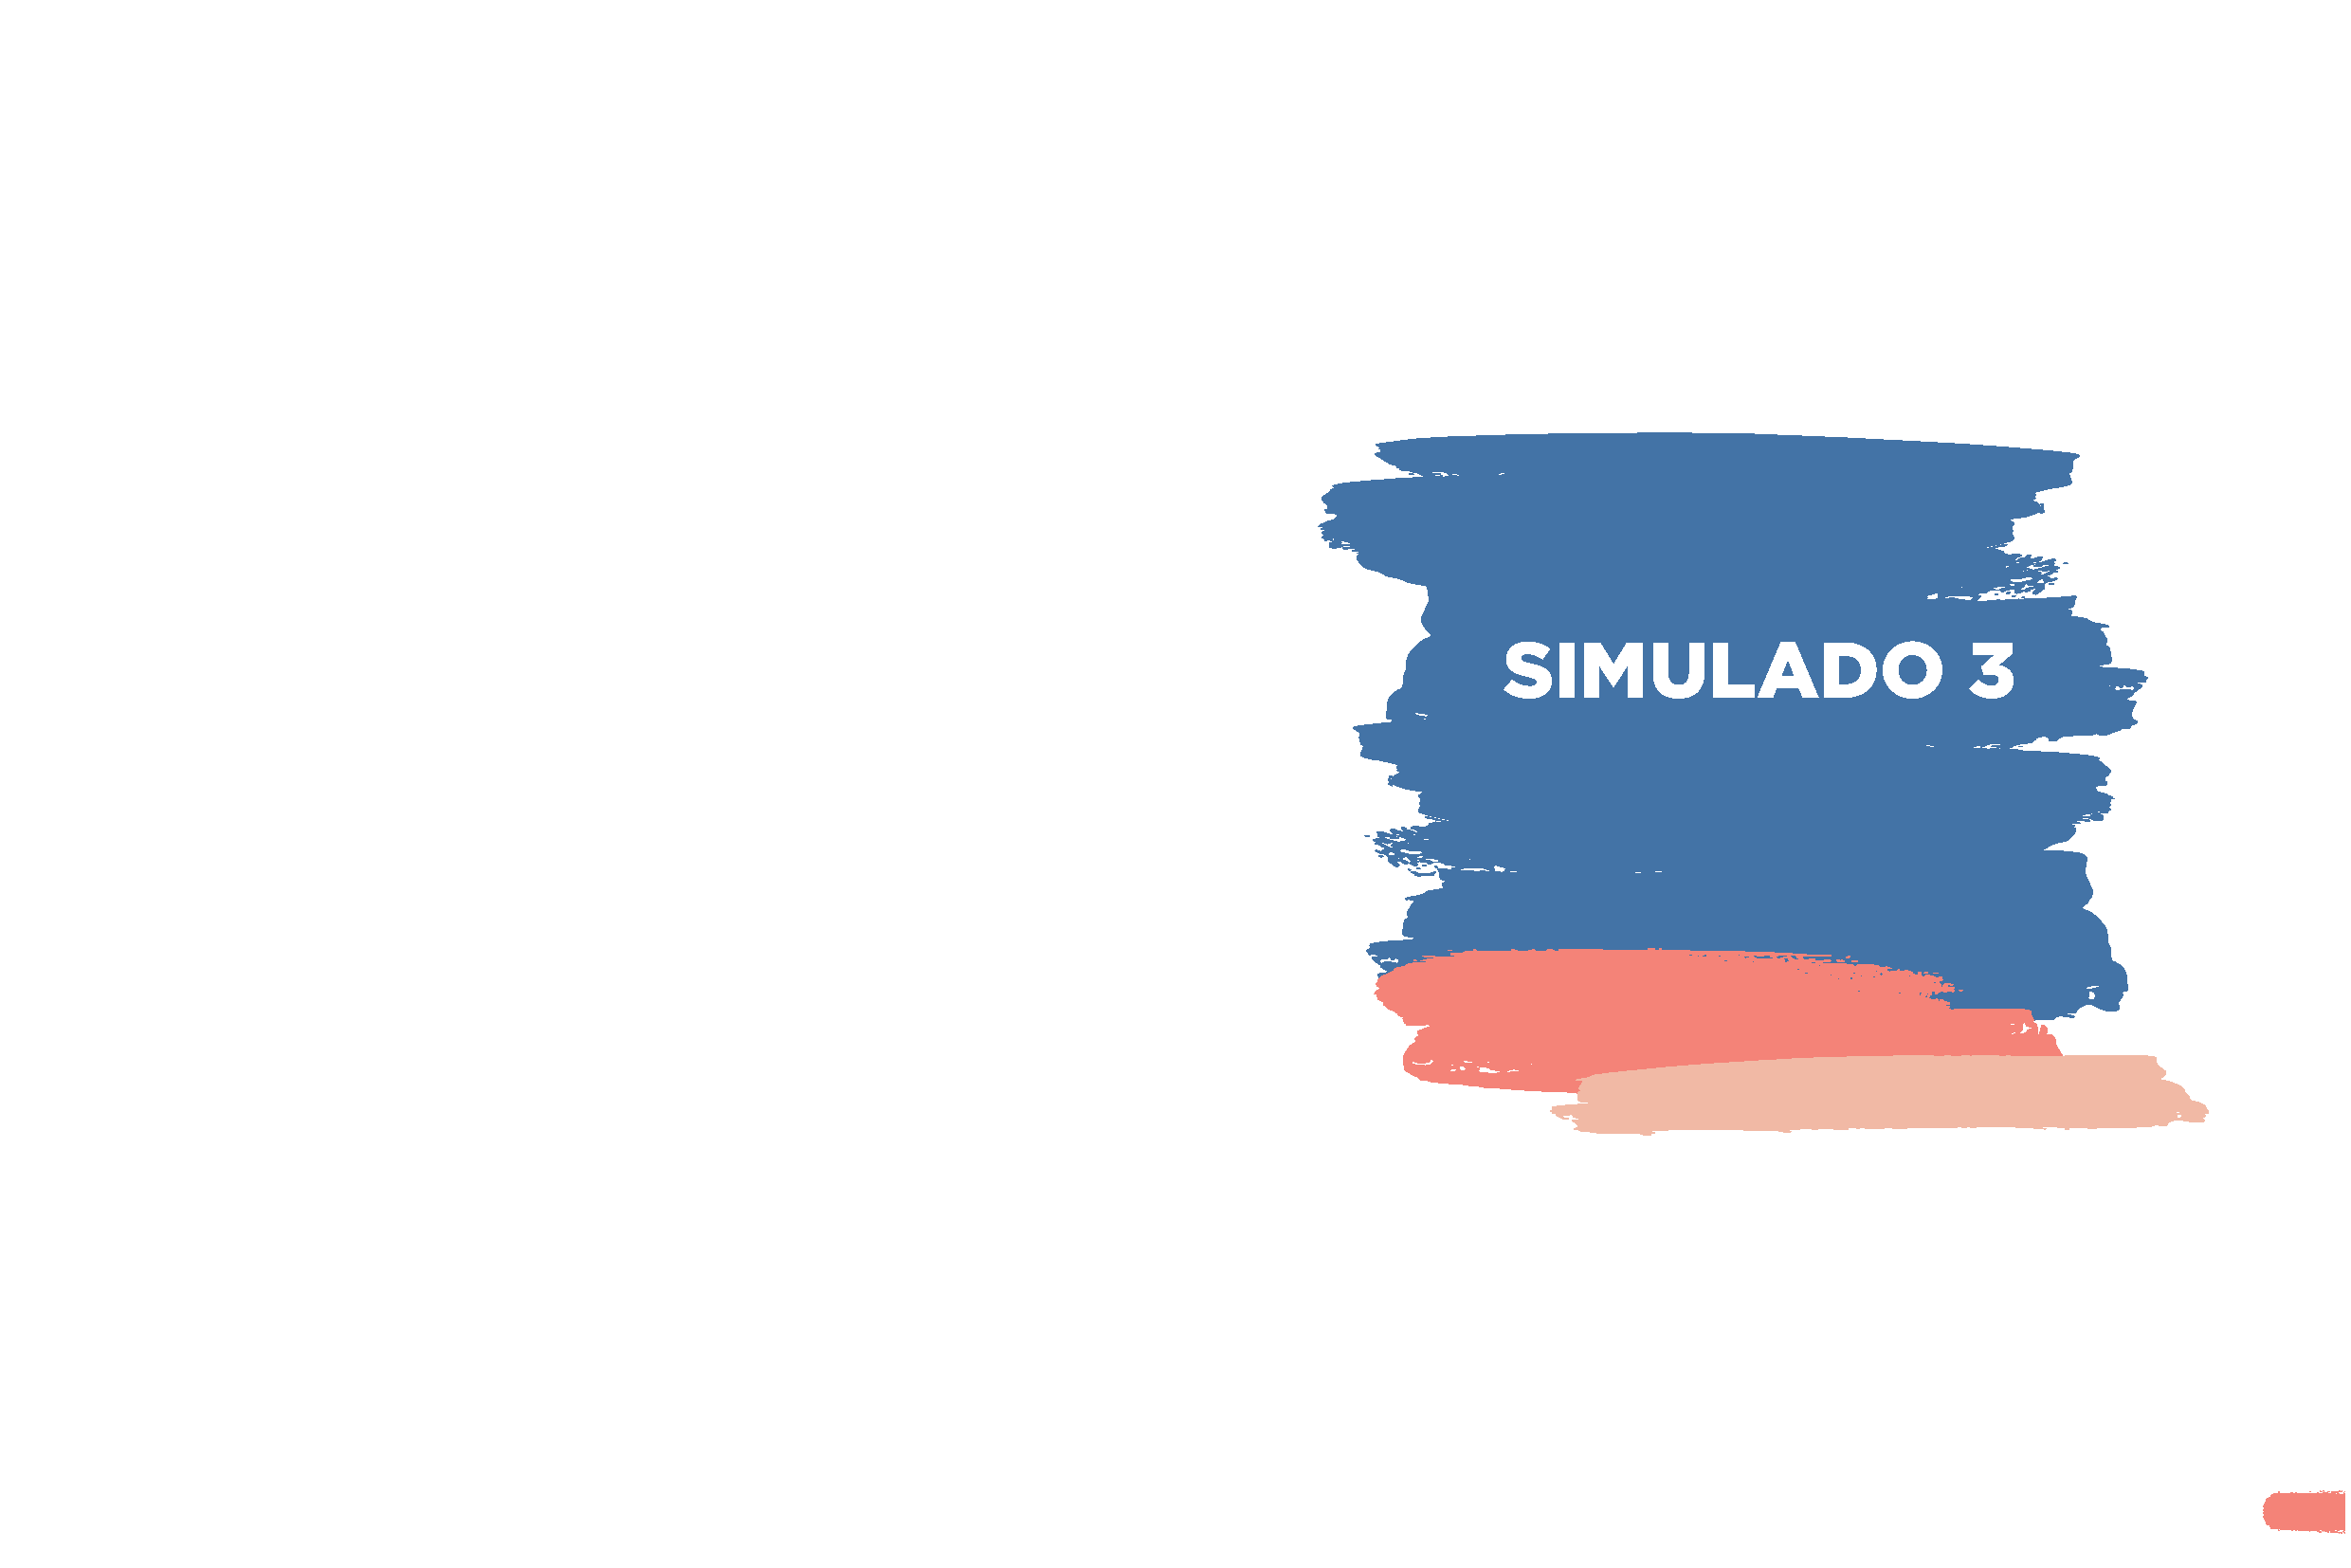
\includegraphics[scale=1]{../watermarks/3simulado5ano.pdf}
\addcontentsline{toc}{chapter}{Simulado 3}
\markboth{Simulado 3}{}

\num{1} As instruções de jogos são textos que apresentam o passo a passo
de como realizar o jogo. Se alterarmos algo, as informações e os objetivos
mudam, assim como a forma de jogar. É preciso ler as regras e descobrir
como se joga e, depois, jogar.

Qual é o elemento fundamental nas instruções de jogos?

\begin{escolha}
\item Modo de preparar.

\item Penalizar o perdedor.

\item Definir um vencedor.

\item Imagens das regras definidas.
\end{escolha}

\num{2} Leia o infográfico a seguir.

\begin{figure}[htpb!]
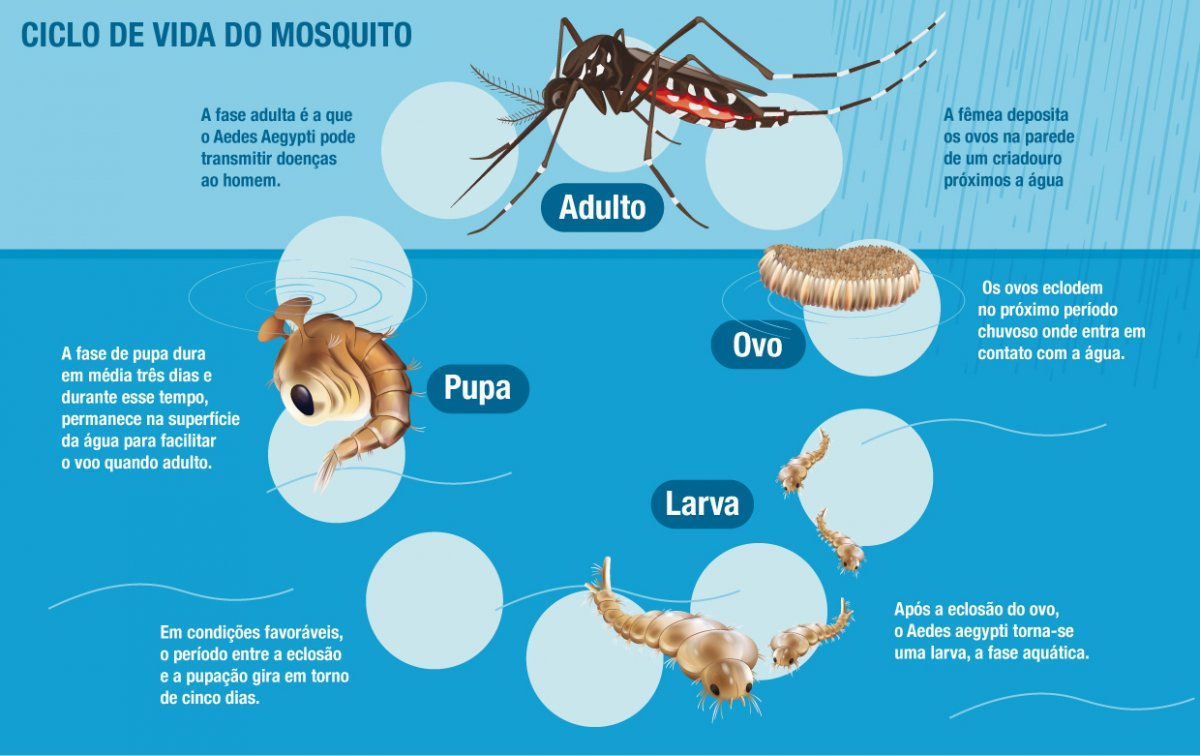
\includegraphics[width=\textwidth]{media/image37.jpeg}
\end{figure}

\fonte{Prefeitura de Santos. Controlar mosquito ajuda a evitar três 
doenças -- confira infográfico. Disponível em:
www.santos.sp.gov.br/?q=content/controlar-mosquito-ajuda-a-evitar-tres-doencas-confira-infografico.
Acesso em: 26 abr. 2023.}

\pagebreak
O infográfico descreve

\begin{escolha}
\item as fases da vida do mosquito \emph{Aedes aegypti}, desde o ovo até a vida adulta.

\item a fase adulta da vida do mosquito \emph{Aedes aegypti}, que costuma durar cinco dias.

\item o momento em que o mosquito \emph{Aedes aegypti} começa a transmitir doenças, ainda como larva.

\item os locais necessários para que o mosquito \emph{Aedes aegypti} se reporduza e transmita doenças.
\end{escolha}

\num{3} Leia o infográfico a seguir.

\begin{figure}[htpb!]
\centering
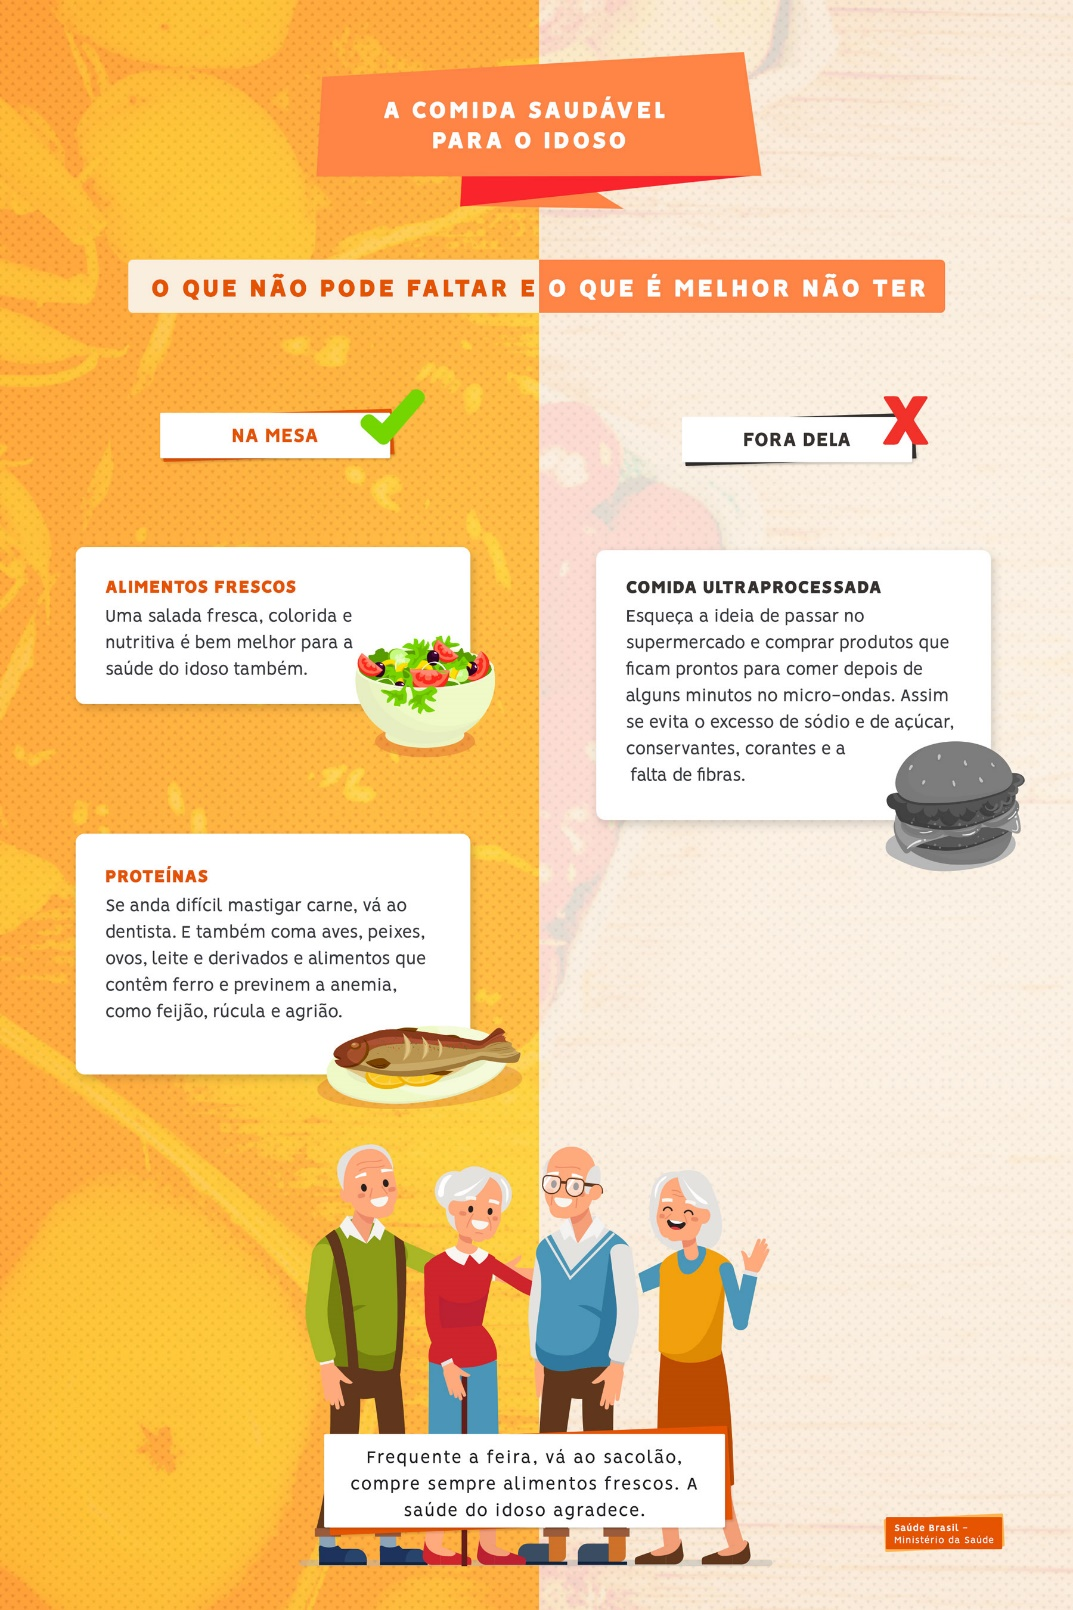
\includegraphics[width=.5\textwidth]{media/image38.jpeg}
\end{figure}

\fonte{Saúde Brasil. Conheça os fatores que influenciam a alimentação de pessoas com mais de
60 anos. Disponível em:
http://saudebrasil.saude.gov.br/eu-quero-me-alimentar-melhor/conheca-os-fatores-que-influenciam-a-alimentacao-de-pessoas-com-mais-de-60-anos.
Acesso em: 19 mar. 2023.}

%Não encontrei essa página de jeito nenhum

Qual é o tema central do infográfico?

\begin{escolha}
\item As proteínas presentes em alimentos que contêm muito sódio.

\item Os tipos de alimentos frescos adequados para o consumo da população.

\item As doenças causadas pelo consumo de alimentos ultraprocessados.

\item Os alimentos saudáveis e os não saudáveis para os idosos.
\end{escolha}

\num{4} Leia o poema abaixo para responder à pergunta.

\begin{quote}
\textbf{Meus oito anos}

\begin{verse}
Oh! que saudades que eu tenho\\
Da \textbf{aurora} da minha vida,\\
Da minha infância querida\\
Que os anos não trazem mais! 
\end{verse}


\fonte{Casimiro de Abreu. Meus oito anos. Disponível em: http://www.pb.utfpr.edu.br/literaturalusofona/Infancia/Casimiro\%20de\%20Abreu/Meus\_oito\_anos\_Casimiro\_de\_Abreu.pdf. Acesso em: 5 mai.2023.}
\end{quote}

No contexto em que está inserida, pode-se afirmar que a palavra destacada
tem o sentido de

\begin{multicols}{2}
\begin{escolha}
  \item início.
  \item fim.
  \item beleza.
  \item tristeza.
\end{escolha} 
\end{multicols}

\pagebreak
\num{5} Leia o texto e responda à pergunta.

\begin{quote}
\textbf{Jovens de até 24 anos veem 7 vezes menos TV aberta do que idosos}

Gabriela Borges, coordenadora do Observatório da Qualidade no
Audiovisual e professora da Universidade do Algarve, confirma essa
tendência.

Ela cita outra pesquisa recente, feita em 2022, pela Ofcom, a agência
reguladora britânica. O levantamento mostra que jovens entre 16 e 24
anos assistem quase sete vezes menos televisão do que pessoas com 65
anos ou mais, passando menos de uma hora em frente à TV.

``Eu acho que esse dado também é importante, porque os jovens já não
assistem a televisão, mas eles migram e eles assistem conteúdo
audiovisual nas plataformas de streaming ou conteúdos \textit{on demand}
e em vídeos de redes sociais''.

\fonte{Agência Brasil. Jovens de até 24 anos veem 7 vezes menos TV 
aberta do que idosos. Disponível em:
https://agenciabrasil.ebc.com.br/geral/noticia/2023-02/jovens-de-ate-24-anos-veem-7-vezes-menos-tv-aberta-do-que-idosos.
Acesso em: 4 mai. 2023}
\end{quote}

O trecho entre aspas encontrado ao final do texto reproduzido acima
indica um(a)

\begin{escolha}
  \item opinião.

  \item fato.

  \item narrativa.

  \item verso.
\end{escolha}

\pagebreak
\num{6} Leia o texto e responda à pergunta.

\begin{quote}
\textbf{Telemedicina chegou com a pandemia e veio para ficar, indica estudo}

Uma pesquisa feita com 1.183 médicos dos Estados de São Paulo e do
Maranhão mostrou que os diversos usos da telemedicina -- que despontaram
como alternativa durante a crise sanitária causada pela COVID-19 --
devem permanecer no sistema de saúde brasileiro.

``Os sistemas de saúde, ao se adaptarem às crises -- econômica, política
ou sanitária --, acabam encontrando soluções e alternativas que podem
ser \textbf{transitórias} ou permanentes. Como nosso projeto de pesquisa
estava em andamento quando veio a pandemia, decidimos, a partir do
estudo do trabalho dos médicos, entender mudanças na saúde que possam
ter sido aceleradas pela COVID-19'', explica o pesquisador à Agência
FAPESP.

\fonte{Governo do Estado de São Paulo. Telemedicina chegou com a
pandemia e veio para ficar, indica estudo. Disponível em:
https://www.saopaulo.sp.gov.br/spnoticias/telemedicina-chegou-com-a-pandemia-e-veio-para-ficar-indica-estudo/.
Acesso em: 24 abr. 2023. com adaptações.}
\end{quote}

A partir do contexto, é possível inferir que o termo destacado se
refere a algo

\begin{escolha}
  \item eterno.

  \item fútil.

  \item de boa qualidade.

  \item passageiro.
\end{escolha}

\pagebreak
\num{7} Leia o texto e responda à pergunta.

\begin{quote}
\textbf{Lugares e monumentos contam a história do 7 de Setembro em São
Paulo}

Foi às margens do riacho Ipiranga, há 199 anos, em um 7 de setembro como
hoje, que Dom Pedro I (1789-1834) declarou a independência do Brasil em
relação a Portugal. O Brasil então se torna uma monarquia e Dom Pedro I
passa a ser imperador.

Em São Paulo, onde a independência foi declarada, diversos museus e
monumentos ajudam a contar essa história e a entender que esse
\textbf{acontecimento} foi um processo e não se encerrou no momento do
grito.

\fonte{Agência Brasil. Lugares e monumentos contam a história do 
7 de Setembro em São Paulo. Disponível em:
https://agenciabrasil.ebc.com.br/geral/noticia/2021-09/lugares-historicos-contam-historia-do-7-de-setembro-em-sp.
Acesso em: 4 mai. 2023.}
\end{quote}

O termo destacado acima refere-se ao/à

\begin{escolha}
  \item grito do Ipiranga.

  \item cidade de São Paulo.

  \item monumentos.

  \item independência do Brasil.
\end{escolha}

\num{8} Leia o texto e responda à pergunta.

\begin{quote}
\textbf{Poluição em São Paulo cai 50\% com a quarentena}

Apesar de todos os problemas acarretados com a pandemia do novo
coronavírus em todo o mundo, a imposição do isolamento social para
controlar o avanço da doença ajudou a reduzir os níveis de poluição nas
grandes cidades, como mostra a reportagem de Daniel Antonio à Agência
FAPESP.

\textbf{Isso acontece porque} a principal fonte de emissão de poluentes é a
frota veicular, que durante a quarentena está menos ativa do que o
normal. A avaliação é da professora do Instituto de Astronomia,
Geofísica e Ciências Atmosféricas da Universidade de São Paulo
(IAG-USP), Maria de Fátima Andrade.

\fonte{Governo do Estado de São Paulo. Poluição em São Paulo cai 50\% com a quarentena. Disponível em:
https://www.saopaulo.sp.gov.br/noticias-coronavirus/poluicao-em-sao-paulo-cai-50-com-a-quarentena/.
Acesso em: 4 mai. 2023. com adaptações.}
\end{quote}

O trecho destacado acima apresenta uma causa para

\begin{escolha}
  \item o aumento da poluição na cidade de São Paulo.

  \item a diminuição das taxas de poluição na cidade de São Paulo.

  \item a transmissão do coronavírus na cidade de São Paulo.

  \item o aumento na frota de veículos na cidade de São Paulo.
\end{escolha}

\num{9} Leia o texto e responda à pergunta.

\begin{quote}
\textbf{Tributo a Guilherme de Almeida revela as várias facetas do 
escritor}

O museu Casa Guilherme de Almeida realiza no mês de julho mais uma
edição do \textit{Guilherme de Almeida em Cena} -- evento que homenageia a obra
do poeta em seu mês de nascimento e falecimento. A atividade, que
acontece de 21 a 24 de julho, tem como objetivo apresentar a pluralidade
do trabalho do escritor e contempla desde sua atuação como cronista e
crítico de cinema até seu interesse pela cultura japonesa,
principalmente pelo haicai -- modelo de poema de origem japonesa que tem
a brevidade como uma de suas características. Neste ano a programação
abre as inscrições para as atividades presenciais e virtuais.

O tributo inicia no dia 21 de julho, quinta-feira, a partir das 19h, com
a palestra ``Crônicas de Guilherme de Almeida'', de Cesar Veneziani,
poeta e mestre em Estudos da Tradução pela FFLCH-USP, e Marlene Laky,
jornalista pela PUC-CAMP, conservadora-restauradora formada pelo SENAI e
coordenadora de oficinas sobre conservação de livros na Casa Guilherme
de Almeida.

\fonte{Disponível em: Governo do Estado de São Paulo. Tributo a
Guilherme de Almeida revela as várias facetas do escritor
Disponível em: https://www.saopaulo.sp.gov.br/ultimas-noticias/tributo-a-guilherme-de-almeida-revela-as-varias-facetas-do-escritor/.
Acesso em: 24 abr. 2023.}
\end{quote}

O texto reproduzido acima fala sobre

\begin{escolha}
  \item uma homenagem ao poeta Guilherme de Almeida.

  \item a necessidade de mais eventos literários serem realizados.

  \item os poemas mais importantes do escritor Guilherme de Almeida.

  \item a tradução de poemas no Brasil.
\end{escolha}


\num{10} Leia o texto e responda à pergunta.

\begin{quote}
\textbf{Governo da Bahia reforça combate às fake news via WhatsApp}

O Governo do Estado amplia as ações de combate à desinformação com mais
um canal para denúncias de notícias falsas e conteúdos enganosos que
circulam pela internet. Através do WhatsApp, os usuários podem mandar
mensagens de texto, áudios, imagens ou vídeos para o número (71)
9646-4095. Desde 2020, os baianos e baianas contam também com o site
www.bahiacontraofake.ba.gov.br no enfrentamento às fake news.

As informações enviadas são analisadas pela equipe da Secretaria de
Comunicação Social do Estado (Secom) e encaminhadas para os órgãos
competentes. Após apuração, os esclarecimentos são feitos por meio da
seção ``Fato ou Fake'' do site. A plataforma pioneira do governo baiano
disponibiliza ainda artigos e vídeos que abordam a temática da
desinformação e os efeitos da disseminação de notícias falsas.

\fonte{Governo do Estado da Bahia. Governo da Bahia reforça combate 
às fake news via WhatsApp. Disponível em:
https://www.bahia.ba.gov.br/2023/01/noticias/comunicacao/governo-da-bahia-reforca-combate-as-fake-news-via-whatsapp/.
Acesso em: 4 mai. 2023.}
\end{quote}

De acordo com o texto, uma das ações do governo da Bahia para combater
as \textit{fake news} consiste em

\begin{escolha}

  \item criar secretarias competentes para analisar as notícias.

  \item apreender os aparelhos envolvidos na disseminação de notícias
falsas.

  \item aumentar a fiscalização das redes sociais utilizadas no estado.

  \item analisar as informações e encaminhá-las aos órgãos competentes.
\end{escolha}



\num{11} Leia o texto e responda à pergunta.

\begin{quote}
\textbf{Prêmio literário para mulheres é lançado no Planalto}

O governo federal lançou nesta quarta-feira (5) o Prêmio Carolina Maria
de Jesus de Literatura Produzida por Mulheres 2023. O edital prevê a
seleção de 40 obras escritas exclusivamente por mulheres no valor de R\$
50 mil por agraciada, totalizando R\$ 2 milhões.

Pelo menos 20\% das obras selecionadas deverão ser escritas por mulheres
negras. Cotas para autoras indígenas, quilombolas, ciganas e com
deficiência também estão previstas. Os gêneros literários aceitos serão
\textbf{conto, crônica, romance, quadrinho e roteiro de teatro}. As
inscrições deverão ser realizadas no site da Ministério da Cultura de 12
de abril a 10 de junho.

\fonte{Agência Brasil. Prêmio literário para mulheres é lançado no 
Planalto. Disponível em:
https://agenciabrasil.ebc.com.br/geral/noticia/2023-04/premio-literario-para-mulheres-e-lancado-no-planalto.
Acesso em: 4 mai. 2023.}
\end{quote}

No trecho destacado, a vírgula é utilizada para

\begin{escolha}
  \item destacar uma informação.

  \item pontuar uma dúvida.

  \item enumerar diferentes informações.

  \item concluir uma frase.
\end{escolha}

\num{12} Leia o texto e responda à pergunta.

\begin{quote}
\begin{verse}
\textbf{Flores luxemburguesas}

Não é, não é alegria,\\
Nem é tristeza sombria\\
Que sinto me atravessar.\\
Grato, grato sentimento\\
De um passado encantamento ---\\
Por toda parte a lembrar!

Eram as roxas florestas,\\
As sagradas sombras mestas\\
Nossos berços da soidão:\\
Se deles tendes as flores, ---\\
A saudade dos amores\\
Em vós reconheço estão.
\end{verse}

%\fonte{Sousândrade. Flores Luxemburguesas. Disponível em: https://www.literaturabrasileira.ufsc.br/documentos/?action=download\&id=43476\#02. Acesso em: 4 mai. 2023.}
\end{quote}

\pagebreak
O poema reproduzido acima apresenta

\begin{escolha}
  \item 12 estrofes.

  \item 6 estrofes.

  \item 1 estrofe.

  \item 2 estrofes.
\end{escolha}


\num{13} Observe a imagem e responda à pergunta.

\begin{figure}[htpb!]
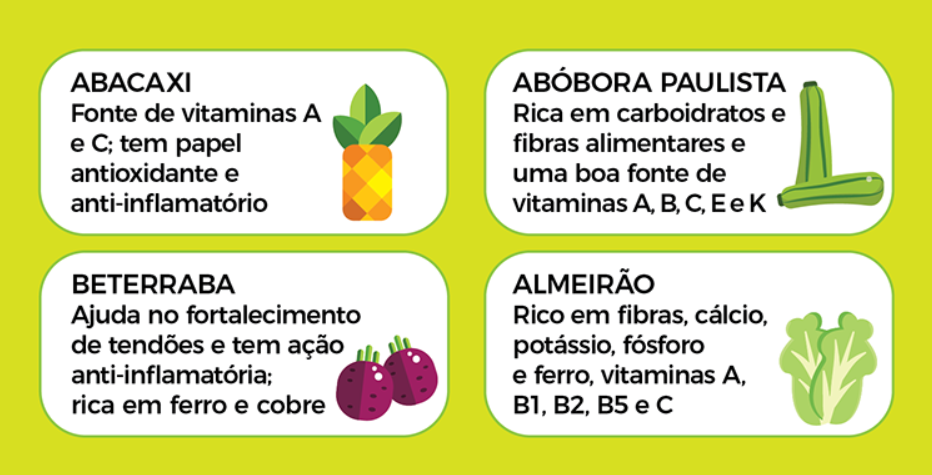
\includegraphics[width=\textwidth]{./imgQ4PORT/media/image4.png}
\end{figure}

\fonte{Governo de São Paulo. Conheça alguns dos alimentos típicos 
da primavera Disponível em:
https://www.saopaulo.sp.gov.br/spnoticias/conheca-alguns-dos-alimentos-tipicos-da-primavera/.
Acesso em: 4 mai. 2023.}

De acordo com o infográfico, um dos benefícios da beterraba é

\begin{escolha}
  \item sua ação antioxidante.

  \item sua ação anti-inflamatória.

  \item a presença de vitamina A.

  \item a presença de muitas fibras.
\end{escolha}

\pagebreak
\num{14} Leia o texto e responda à pergunta.

\begin{quote}
Camilo pegou-lhe nas mãos, e olhou para ela sério e fixo. Jurou que lhe
queria muito, que os seus sustos pareciam de criança; em todo o caso,
quando tivesse algum receio, a melhor cartomante era ele mesmo. Depois,
repreendeu-a; disse-lhe que era imprudente andar por essas casas. Vilela
podia sabê-lo, e depois \ldots

\fonte{Machado de Assis. A Cartomante. Disponível em:
https://machado.mec.gov.br/obra-completa-lista/item/download/26\_29eaa69154e158508ef8374fcb50937a.
Acesso em: 4 mai. 2023.}
\end{quote}

O trecho reproduzido acima apresenta a fala de/do

\begin{escolha}
  \item Machado de Assis.

  \item narrador.

  \item Camilo.

  \item Vilela.
\end{escolha}


\pagebreak
\num{15} Observe a imagem e responda à pergunta.

\begin{figure}[htpb!]
\centering
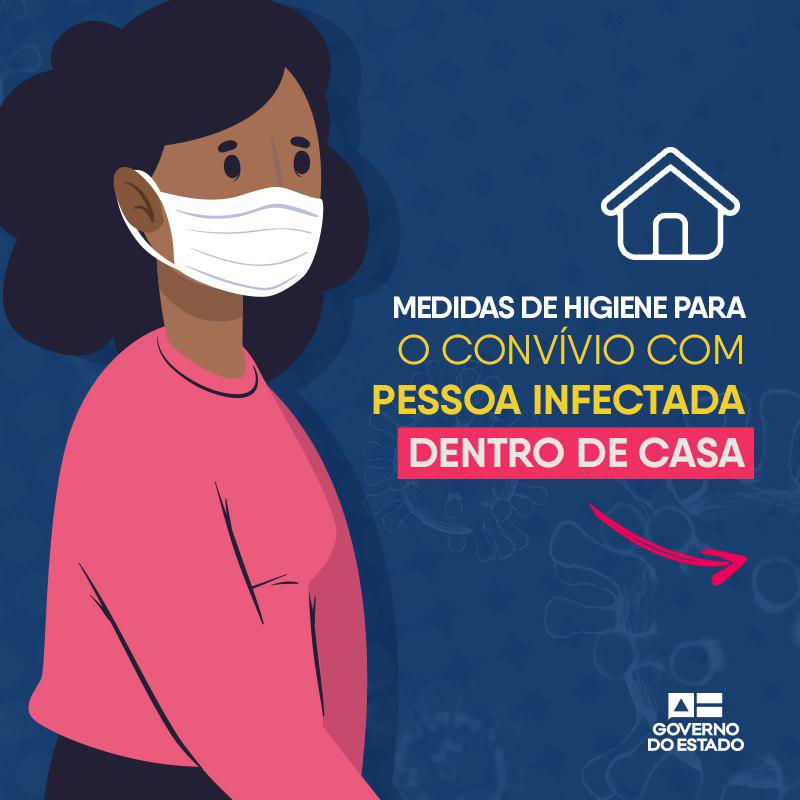
\includegraphics[width=.8\textwidth]{./imgQ4PORT/media/image5.jpeg}
\caption{Uma imagem contendo Diagrama Descrição gerada automaticamente}
\end{figure}

\fonte{Disponível em: Secretaria da Saúde do Governo do Estado da Bahia.
Peças de Campanha – Covid-19. 
https://www.saude.ba.gov.br/temasdesaude/coronavirus/campanhacovid19/>.
Acesso em: 4 mai. 2023.}

De acordo com a ilustração reproduzida acima, podemos inferir que

\begin{escolha}
  \item o uso de máscaras é necessário.

  \item a higiene não combate o vírus.

  \item não é preciso preocupar-se com a infecção.

  \item o uso de máscaras é opcional.
\end{escolha}


\vspace*{-3.4cm}
\hspace*{-3.7cm}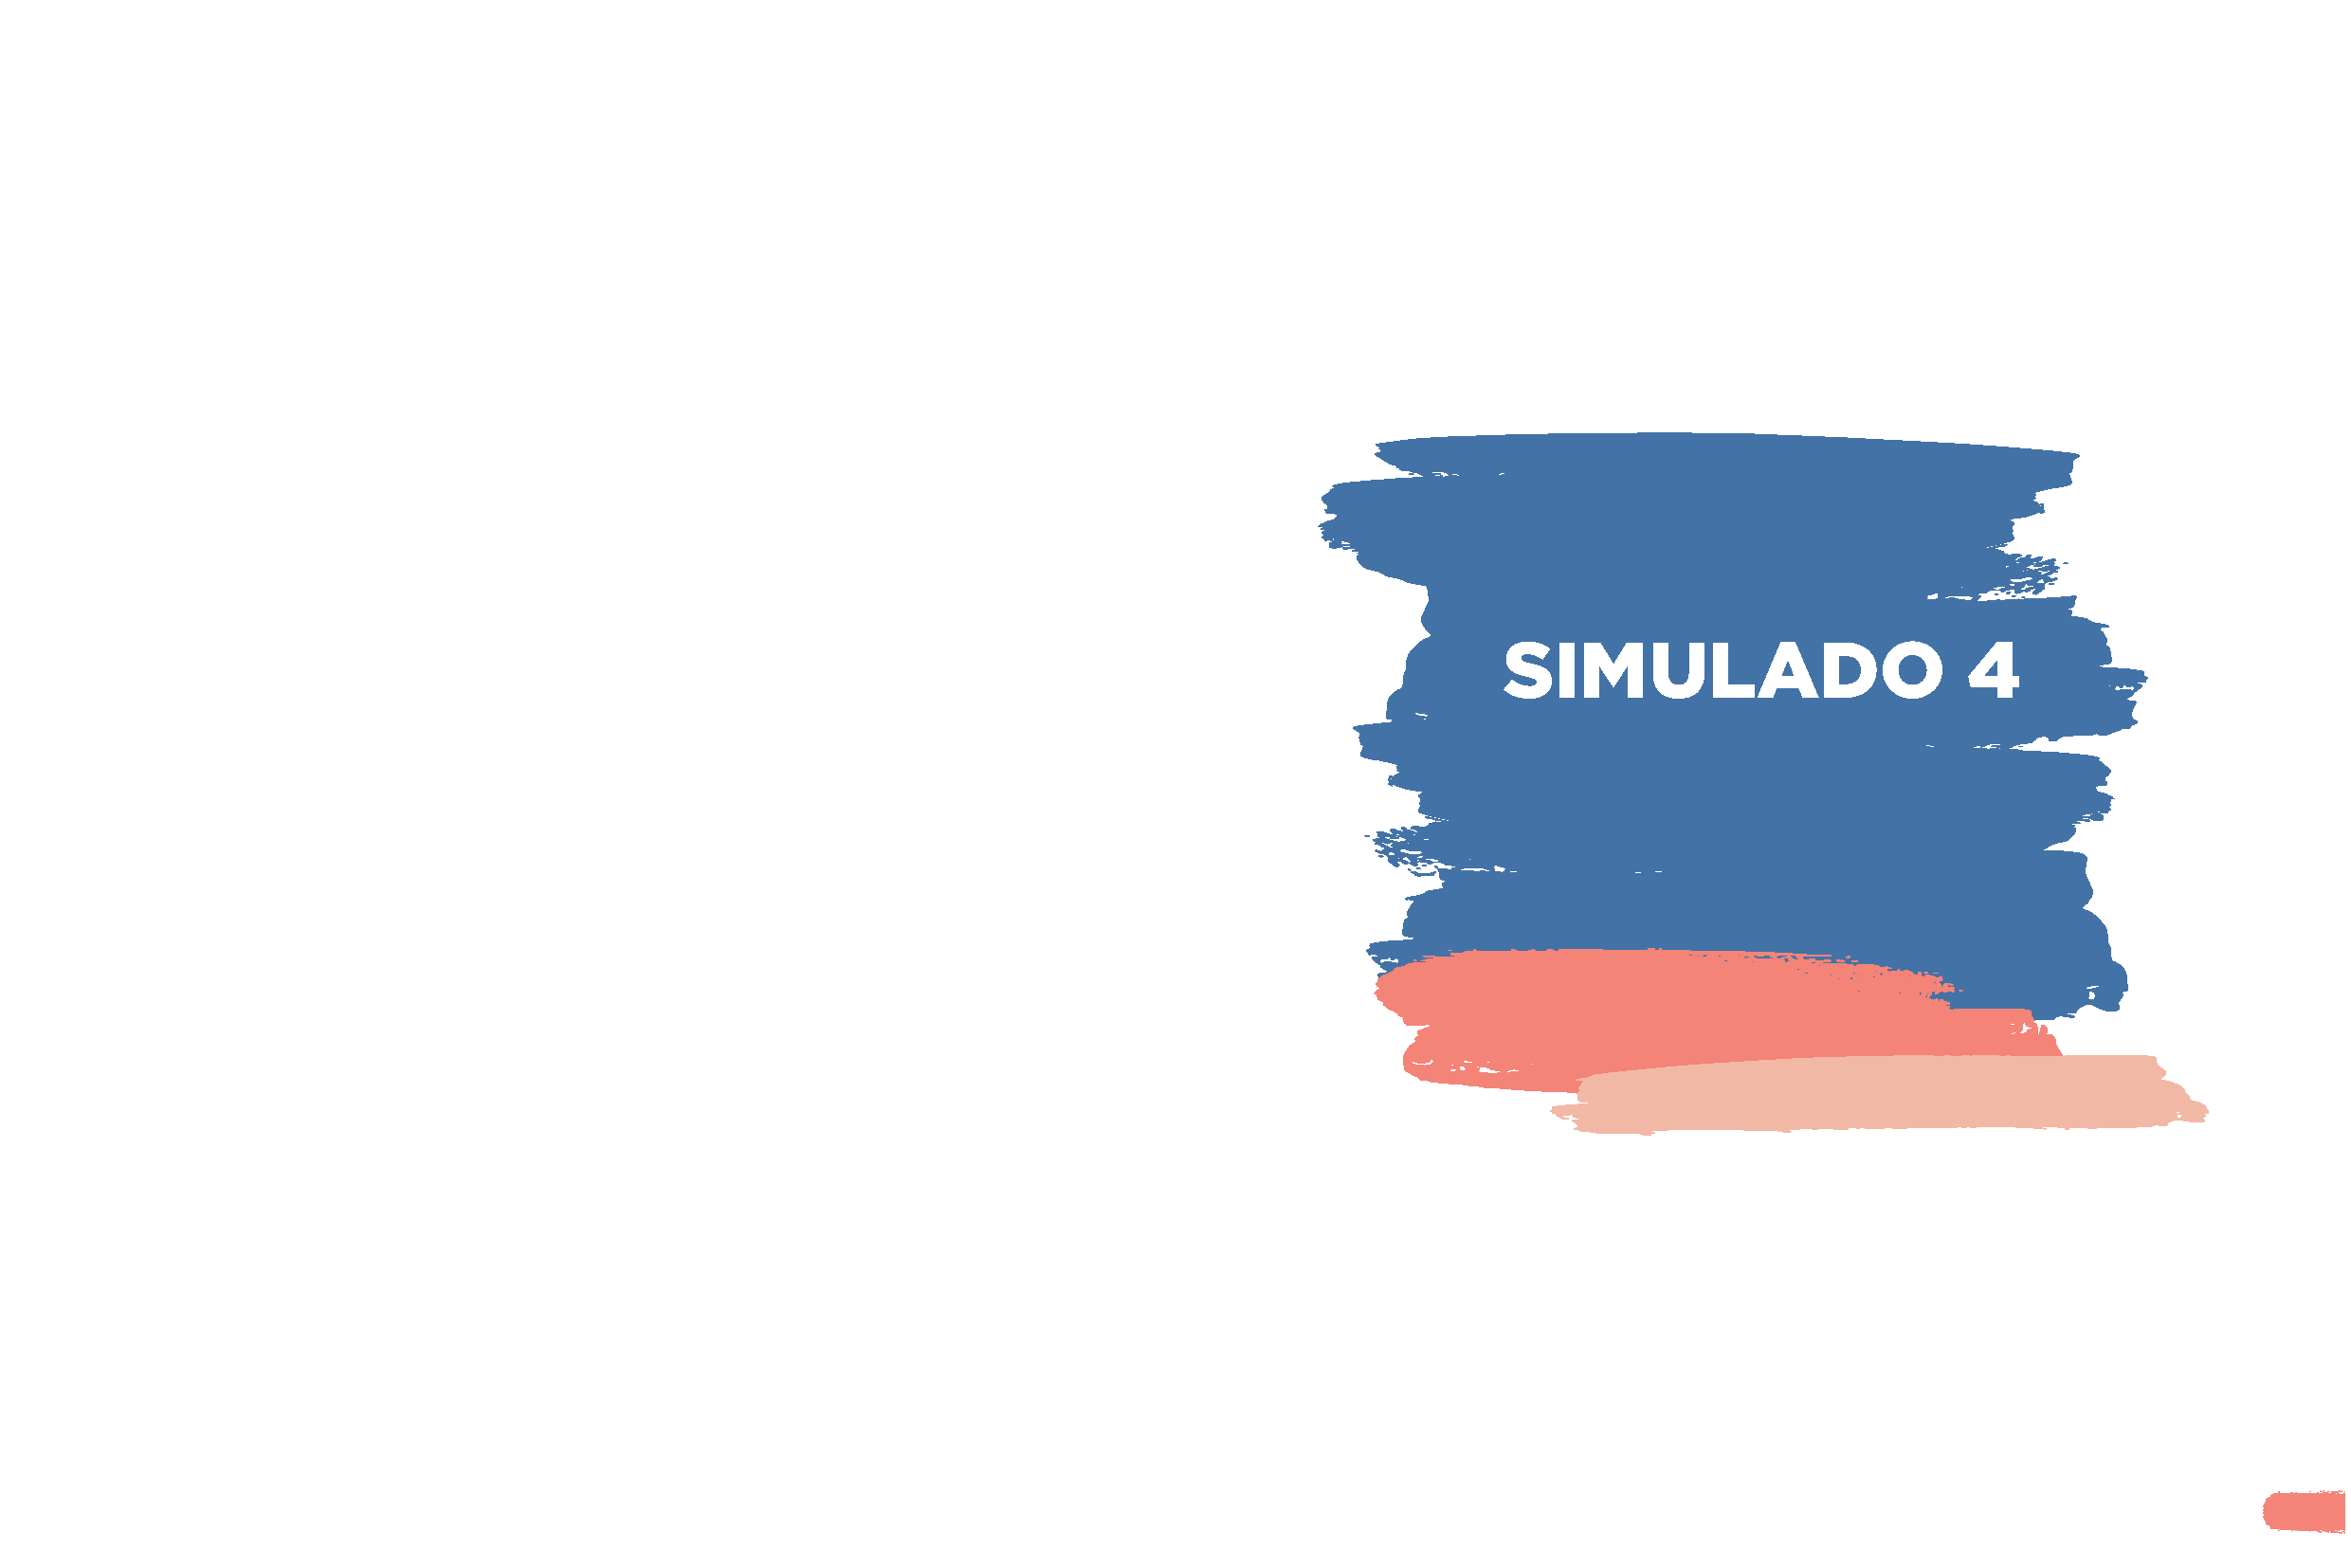
\includegraphics[scale=1]{../watermarks/4simulado5ano.pdf}
\addcontentsline{toc}{chapter}{Simulado 4}
\markboth{Simulado 4}{}

\num{1} Leia um trecho do conto a seguir.

\begin{quote}
\textbf{O asno, o boi e o lavrador}

Um lavrador muito rico tinha várias casas no campo onde criava muitos
animais. Vivia em uma delas com a mulher e seus filhos. Ele possuía,
como Salomão, o dom de entender a língua em que falavam os animais,
embora não lhe fosse permitido traduzir o que ouvia às outras pessoas,
sob pena de perder a vida.

Tinha no mesmo curral um boi e um asno e, certo dia, enquanto observava
as brincadeiras de seus filhos, ouviu o boi dizer ao asno:

--- Não posso deixar de invejar tua sorte, ao ver o muito que descansas e
o pouco que trabalhas. Há um empregado que cuida de ti, te dá boa cevada
para comeres e água cristalina para beberes; e se não fossem as poucas
vezes que levas nosso dono nas curtas viagens que faz, passarias a vida
de pernas para o ar. Já a mim, tratam de modo diferente, sendo minha
situação tão desgraçada quanto é agradável a tua. Mal começa o dia, me
prendem a uma carreta, trabalho até não ter mais forças, e o lavrador,
além disso, me espanca sem parar, dando-me depois para comer algumas
favas secas. Vês que tenho razão de invejar tua sorte.

\fonte{O asno, o boi e o lavrador. \textit{As mil e uma noites: contos
árabes}. Rio de Janeiro: Revan, set. 2010. 5. ed. p. 15-16.}
\end{quote}

Na opinião do boi, o asno

\begin{escolha}
\item entende facilmente a língua falada pelo dono.

\item trabalha demais, pois sempre acompanha o dono nas viagens

\item tem uma vida tranquila, por não precisar trabalhar tanto.

\item é muito mais forte porque se alimenta de boa cevada.
\end{escolha}

\pagebreak
\num{2} Leia o trecho do conto ``As mil e uma noites''.

\begin{quote}
Finalmente chegaram a uma região montanhosa, que era
exatamente o lugar onde o falso tio desejava pôr em prática o plano que
o fizera vir de um ponto extremo da África.

--- Já chegamos --- disse ele a Aladin. --- E aqui poderás ver coisas
maravilhosas nunca vistas por nenhum mortal. Agora, junta algumas ervas
secas para acendermos uma fogueira.

Assim que as ervas começaram a queimar, o mágico derramou sobre elas
gotas de um perfume que trazia consigo, fazendo subir da fogueira uma
fumaça espessa, enquanto pronunciava palavras estranhas que Aladin não
compreendia. Nesse momento, a terra estremeceu e se abriu diante dos
dois, deixando ver uma pedra quadrada de mais ou menos 60 centímetros de
lado e 30 centímetros de espessura, tendo ao centro uma argola de metal
que servia para levantá-la. Aladin, assustado com o que acontecia,
tentou fugir, mas foi detido pelo mágico, que o atingiu com um soco no
rosto, tão forte que o derrubou. Aladin, chorando, falou:

--- Tio, que fiz eu para me baterdes deste modo?

--- Tenho minhas razões. Sou teu tio e faço as vezes de teu pai, de modo
que tens de me obedecer. Mas, meu caro sobrinho, se fizerdes exatamente
o que eu mando serás muito bem recompensado.

Essas palavras aliviaram um pouco o temor e o ressentimento de Aladin.

\fonte{A história de Aladin e a lâmpada
maravilhosa. \emph{As mil e uma noites: contos árabes}. Rio
de Janeiro: Revan, set. 2010. 5. ed. p. 144.}
\end{quote}

\pagebreak
De acordo com o trecho, o mágico está

\begin{escolha}
\item mostrando-se assustado com as palavras inteligíveis pronunciadas pelo sobrinho.

\item apresentando coisas maravilhosas a Aladin, com a finalidade de aprofundar laços afetivos.

\item ajudando o sobrinho Aladin, ensinando-o a fazer magias na região extrema da África.

\item fingindo ser o tio de Aladin, apenas para o atrair e poder dar início aos seus planos.
\end{escolha}


\num{3} Leia, a seguir, o trecho de uma notícia que aborda o Dia do
Cooperativismo.

\begin{quote}
\textbf{Dia do Cooperativismo é celebrado em várias cidades brasileiras}

``O cooperativismo trabalha na linha de frente do
desenvolvimento socioeconômico do país. E o Dia de Cooperar é uma forma
de expressar a força do nosso movimento, que por meio de ações
voluntárias, ajuda pessoas a transformarem suas vidas'', afirma o
presidente do Sindicato e Organização das Cooperativas do Estado do Rio
(OCB/RJ), Vinícius Mesquita.

\fonte{Vitor Abdala. Agência Brasil. Dia do Cooperativismo é celebrado em várias cidades
brasileiras. Disponível em:
http://agenciabrasil.ebc.com.br/economia/noticia/2019-07/dia-do-cooperativismo-e-celebrado-em-varias-cidades-brasileiras. Acesso em: 26 abr. 2023. com alterações.}
\end{quote}

No trecho, o autor insere a declaração de uma pessoa com a intenção de

\begin{escolha}
\item dar credibilidade à notícia.

\item dar destaque a aspectos importantes.

\item fazer um complemento ao título.

\item ilustrar o que foi relatado.
\end{escolha}

\pagebreak
\num{4} Leia o trecho retirado de uma entrevista com um aluno de 7 anos
de idade sobre futebol do jornal Folha de S. Paulo.

\begin{quote}
Estudante da escola pública estadual Professor Laerte Panighel, o garoto
de 7 anos se revelou esperto desde a primeira visita da reportagem ao
colégio.

\textbf{Por que tem muito corintiano nessa escola?}

Porque o Corinthians tá ganhando de todos os times. O Palmeiras perdeu
de 1 x 0. Então aqui o Corinthians é mais participado, se o
Palmeiras ganhar vai ser todo mundo ser palmeirense.

\textbf{Ah, o time depende de se está ganhando ou não...}

É. É todo mundo assim. Menos eu. Eu sou só corintiano. Nem que perca,
nem que ganhe.

\fonte{Fábio Victor. Folha de S. Paulo. Não importa para que time você
torce, o que importa é a amizade'', diz Ryan, 7.  Disponível em:
\&lt;http://temas.folha.uol.com.br/crianca-do-dia/esporte/nao-importa-pra-que-time-voce-torce-o-que-importa-e-a-amizade-diz-ryan-7.shtml\&gt;.
Acesso em: 19 mar. 2023.}
\end{quote}

Conforme informações do texto, o aluno

\begin{escolha}
\item muda de time a cada partida, torcendo sempre para o vencedor.

\item torce para o mesmo time que a maioria da escola, o Palmeiras.

\item não entende por que seus colegas mudam de time o tempo todo.

\item gosta muito do mesmo time e não muda sua torcida por nada.
\end{escolha}



\num{5} Leia o texto e responda à pergunta.

\begin{quote}
\textbf{Mais livros: governo quer retomar políticas públicas para leitura}

Fazer uma nação leitora, este é o desafio do atual governo. Em
entrevista exclusiva para a Agência Brasil, o secretário de Formação,
Livro e Leitura do Ministério da Cultura, Fabiano Piúba, destaca as
ações de retomada das políticas para a área, assim como aponta propostas
da pasta para o novo Programa de Aceleração do Crescimento (PAC). De
acordo com ele, a formação leitora dos brasileiros é uma das prioridades
da gestão.

\textbf{Além disso}, existe a expectativa de destacar recursos orçamentários
para o programa de tradução de obras de autores brasileiros, coordenado
pela Fundação Biblioteca Nacional. Dessa forma, a pasta espera
repercutir nossa criação literária em línguas diversas.

\fonte{Agência Brasil. Mais livros: governo quer retomar políticas 
públicas para leitura. Disponível em:
https://agenciabrasil.ebc.com.br/geral/noticia/2023-04/mais-livros-governo-quer-retomar-politicas-publicas-para-leitura.
Acesso em: 5 mai. 2023. com adaptações.}
\end{quote}

A expressão destacada no trecho acima cumpre a função de

\begin{escolha}
  \item concluir as informações apresentadas no texto.

  \item contrastar dados de duas partes diferentes do texto.

  \item indicar que haverá acréscimo às informações anteriores.

  \item negar as informações discutidas no início do texto.
\end{escolha}



\num{6} Observe a imagem e responda à pergunta.

\begin{figure}[htpb!]
\centering
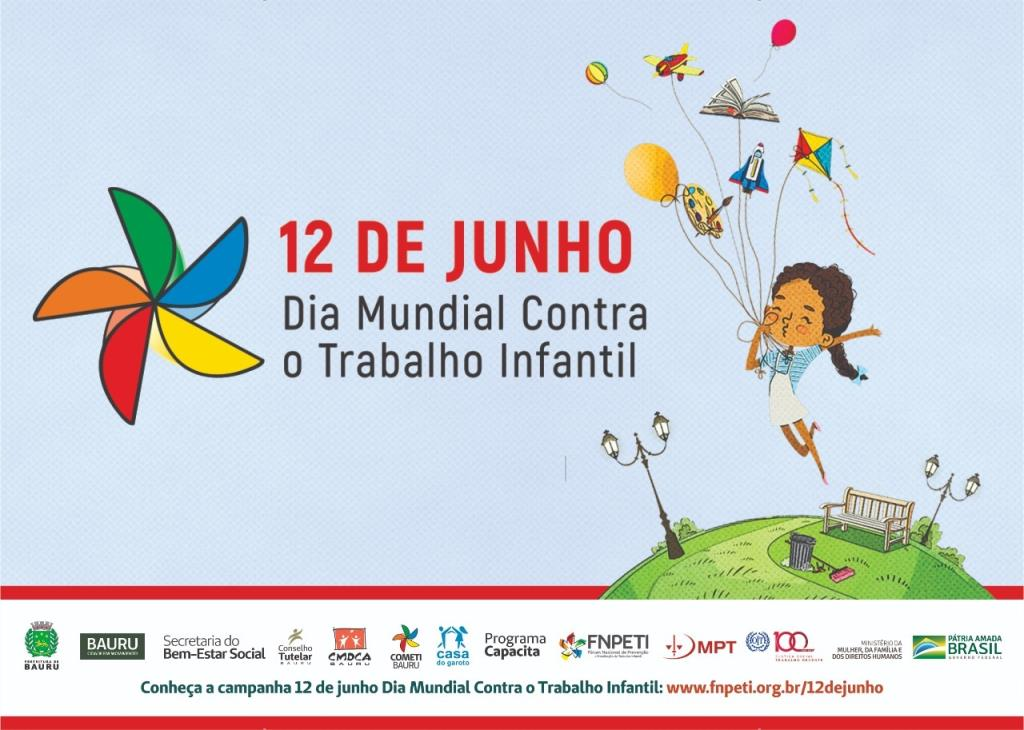
\includegraphics[width=.5\textwidth]{./imgQ4PORT/media/image6.jpeg}
\caption{Diagrama Descrição gerada automaticamente com confiança média}
\end{figure}

\fonte{Prefeitura de Bauru. Prefeitura realiza campanha do Dia Mundial
Contra o Trabalho Infantil. Disponível em: https://www2.bauru.sp.gov.br/materia.aspx?n=34083. Acesso em: 5 mai. 2023.}

Um dos recursos utilizados no cartaz para convencer o leitor da
importância do combate ao trabalho infantil é

\begin{escolha}
  \item a presença de citações de especialistas.

  \item o excesso de textos informativos.

  \item a apresentação de dados estatísticos.

  \item a ilustração de uma garotinha feliz.
\end{escolha}

\num{7} Leia o texto e responda à pergunta.

\begin{quote}
Araci tomou o arco e entrou na floresta. A imagem do guerreiro
\textbf{amado} fugia naquele instante de seus olhos; eles buscaram entre as
folhas o sinal de seus passos e não o descobriram.

\fonte{José de Alencar. Ubirajara. Disponível em:
<http://objdigital.bn.br/Acervo\_Digital/Livros\_eletronicos/ubirajara.pdf>.
Acesso em: 25 abr. 2023.}
\end{quote}

O adjetivo destacado no trecho expressa

\begin{escolha}
  \item carinho.

  \item tristeza.

  \item raiva.

  \item oposição.
\end{escolha}


\pagebreak
\num{8} Leia o texto e responda à pergunta.

\begin{quote}
---Ingênuo! respondeu Procópio Dias batendo-lhe alegremente no ombro.
Se eu confesso que ela não está muito estragada é porque não a quero
para mim. É grande demais; e depois, fica muito \textbf{longe} da cidade.
Se fosse mais para baixo\ldots

\fonte{Machado de Assis. Iaiá Garcia. Disponível em:
https://machado.mec.gov.br/obra-completa-lista/item/download/17\_bff5cb6c81c213a22c492d69505ac411. Acesso em: 5 mai. 2023.}
\end{quote}

O termo destacado no texto é classificado como advérbio de

\begin{multicols}{2}
\begin{escolha}
  \item intensidade.

  \item tempo.

  \item lugar.

  \item modo.
\end{escolha}
\end{multicols}


\num{9} Leia o texto e responda à pergunta.

\begin{quote}
--- Então, uma hora depois do baile? disse eu alçando a voz.

--- Sim; mas segredo! respondeu Nina levando o dedo à boca.

\fonte{José de Alencar. Lucíola. Disponível em:
https://pt.wikisource.org/wiki/Lucíola. Acesso em: 5 mai. 2023.}
\end{quote}

No trecho reproduzido acima, os dois verbos usados para se referir às
falas das personagens são

\begin{escolha}
  \item ``respondeu'' e ``levando''.

  \item ``disse'' e ``respondeu''.

  \item ``levando'' e ``alçando''.

  \item ``alçando'' e ``disse''.
\end{escolha}


\pagebreak
\num{10} Observe a imagem e responda à pergunta.
 
\begin{figure}[htpb!]
\centering

\includegraphics[width=.5\textwidth]{./imgQ4PORT/media/image7.jpeg}
\caption{Interface gráfica do usuário Descrição gerada automaticamente}
\end{figure}

\fonte{Prefeitura Municipal de Delta. Vacine-se contra a gripe 
–- Influenza. Disponível em: https://www.delta.mg.gov.br/vacine-se-contra-a-gripe-influenza/.
Acesso em: 5 mai. 2023.}

O fato de a imagem apresentar diversas pessoas no mesmo espaço sugere
que

\begin{escolha}
  \item a vacinação contra gripe é facultativa.

  \item a vacinação não é uma preocupação da saúde pública.

  \item a vacinação é para diversos setores da população.

  \item a vacinação contra a gripe tem um público-alvo restrito.
\end{escolha}

\num{11} Leia o texto e responda à pergunta.

\begin{quote}
D. LEOCÁDIA (\textit{pegando-lhe nas mãos}) --- Olhe bem para mim. 
(\textit{Pausa}). Suspire. (\textit{Cavalcante suspira}). O senhor está
doente: não negue que está doente --- moralmente, entenda-se; não negue!
(\textit{Solta-lhe as mãos}).

\fonte{Machado de Assis. Não Consultes Médico. Disponível em:
https://machado.mec.gov.br/obra-completa-lista/item/download/66\_390921fb4791464b4885563dc04a042c.
Acesso em: 5 mai. 2023.}
\end{quote}

No trecho acima, as informações entre parênteses apresentam

\begin{escolha}
  \item as falas das personagens.

  \item descrições dos figurinos.

  \item as ações das personagens.

  \item descrições do espaço.
\end{escolha}



\num{12} Leia o texto e responda à pergunta.

\begin{quote}
\textbf{Informação e planejamento são chaves para profissionalizar negócios}

Informação e planejamento são as palavras-chaves para quem decide
empreender, seja por necessidade ou por oportunidade de negócio. Colocar
no papel informações básicas sobre o mercado consumidor e os custos são
essenciais para alinhar as expectativas e garantir a sustentabilidade de
uma empresa no longo prazo, em meio à concorrência.

``Se eu colocar as informações da empresa na internet ou nas redes
sociais, o cliente está nesse canal? Ele vai me enxergar ou eu preciso
fazer algum impresso físico e distribuir para que as pessoas saibam que
estou oferecendo aquele serviço? Ou por meio de algum aplicativo eu
consigo que as pessoas me enxerguem?'', explicou o gerente do Sebrae,
sobre as questões a serem respondidas pelo empreendedor.

\fonte{Agência Brasil. Informação e planejamento são chaves para profissionalizar negócios. Disponível em:
https://agenciabrasil.ebc.com.br/economia/noticia/2021-03/informacao-e-planejamento-sao-chaves-para-profissionalizar-negocios.
Acesso em: 5 mai. 2023. com adaptações.}
\end{quote}

As informações veiculadas no trecho acima podem ser consideradas
confiáveis pelo fato de

\begin{escolha}
  \item utilizarem uma linguagem informal.

  \item serem publicadas na internet.

  \item utilizarem uma linguagem complexa.

  \item contarem com a opinião de um especialista.
\end{escolha}

\num{13} Leia o texto e responda à pergunta.

\begin{quote}
--- Os cálculos não são precisos, disse ele, porque o Dr. Bacamarte não
arranja nada. Quem é que viu agora meter todos os doidos dentro da mesma
casa?

\fonte{Machado de Assis. O Alienista. Disponível em:
https://machado.mec.gov.br/obra-completa-lista/item/download/29\_008edfdf58623bb13d27157722a7281e.
Acesso em: 5 mai. 2023.}
\end{quote}

O sinal de pontuação utilizado no final do trecho indica

\begin{escolha}
  \item uma dúvida.

  \item a fala de uma personagem.

  \item a enumeração de diferentes informações.

  \item um trecho destacado.
\end{escolha}

\num{14} Leia o texto e responda à pergunta.

\begin{quote}
\textbf{Exposição virtual apresenta registros das transformações 
da cidade de São Paulo}

O Acervo Artístico-Cultural dos Palácios do Governo do Estado de São
Paulo apresenta a exposição virtual ``Na Paisagem de São Paulo: Rebolo e
o Grupo Santa Helena'', com mais de 30 pinturas de Francisco Rebolo e
integrantes do chamado Grupo Santa Helena que apresentam importantes
registros das transformações da cidade de São Paulo e seus arredores nas
décadas de 1930 e 1940.

Com curadoria de Ana Cristina Carvalho e Lisbeth Rebolo Gonçalves, a
mostra destaca a relevância desses artistas artesões na consolidação do
modernismo brasileiro e nos desdobramentos do impacto cultural causado
pelos primeiros modernistas pós-Semana de Arte Moderna de 1922.

\fonte{Governo de São Paulo. Exposição virtual apresenta registros das 
transformações da cidade de São Paulo. Disponível em:
https://www.saopaulo.sp.gov.br/spnoticias/exposicao-virtual-apresenta-registros-das-transformacoes-da-cidade-de-sao-paulo/.
Acesso em: 5 mai. 2023.}
\end{quote}

O tema do texto reproduzido acima é

\begin{escolha}
  \item o processo de urbanização ocorrido em São Paulo na década de 1940.

  \item os novos movimentos artísticos encontrados na cidade de São Paulo.

  \item uma exposição virtual sobre a cidade de São Paulo.

  \item a Semana de Arte Moderna de 1922.
\end{escolha}

\num{15} Leia o texto e responda à pergunta.

\begin{quote}
\textbf{Estudantes surdos poderão ter acesso a vídeo com prova do Enem
traduzida}

Pela primeira vez, estudantes surdos poderão ter acesso a vídeo com as
questões do Enem traduzidas na Língua Brasileira de Sinais (Libras). O
Instituto Nacional de Estudos e Pesquisas Educacionais Anísio Teixeira
(Inep) vai disponibilizar salas adaptadas, e o participante poderá
escolher, na inscrição, se deseja participar da aplicação.

Os estudantes que optarem pela tradução no vídeo terão também acesso a
um tradutor por dupla de candidatos, que poderá apenas esclarecer
dúvidas pontuais de vocabulário. Eles preencherão o cartão de respostas
normalmente. A disponibilização do vídeo será feita este ano em caráter
experimental.

\fonte{Agência Brasil. Estudantes surdos poderão ter acesso a vídeo com prova do Enem
traduzida. Disponível em:
<https://agenciabrasil.ebc.com.br/educacao/noticia/2017-04/estudantes-surdos-poderao-ter-acesso-video-com-prova-do-enem-traduzida>.
Acesso em: 26 abr. 2023. com adaptações.}
\end{quote}

De acordo com o texto

\begin{escolha}
  \item a iniciativa já foi realizada anteriormente.

  \item estudantes surdos não podem realizar a prova do Enem.

  \item será disponibilizado um vídeo para que os estudantes surdos.

  \item não será disponibilizado um tradutor para os candidatos.
\end{escolha}



\chapter{Referências}
\markboth{Referências}{}

\begin{bibliohedra}
\tit{brasil}. Ministério da Educação. \textbf{Base nacional comum curricular}:
educação é a base.

\tit{brasil}. Ministério da Educação. \textbf{Pacto nacional pela
alfabetização na idade certa}. Disponível em:
\textless{}http://www.serdigital.com.br/gerenciador/clientes/ceel/material/149.pdf\textgreater{}.
Acesso em: fev. 2023.

\tit{kaufman}, Ana María; RODRÍGUEZ, María Helena. \textbf{Escola, leitura e
produção de textos}. Porto Alegre: Artmed, 1995.

\tit{koch}, Ingedore G. Villaça. \textbf{Ler e escrever}: estratégias de
produção textual. São Paulo: Contexto, 2010.

\tit{lerner}, Delia. \textbf{Ler e escrever na escola}: o real, o possível e o
necessário. Porto Alegre: Artmed, 2002.

\tit{nóbrega}, Maria José. \textbf{Ortografia}. São Paulo: Melhoramentos,
2013.
\end{bibliohedra}

\chapter{Sites}
\markboth{Sites}{}

\begin{itemize}
\item\textbf{Ciência Hoje das Crianças}. Disponível em:
http://chc.org.br/. Acesso em: fev. 2023.

\item\textbf{DOMÍNIO PÙBLICO}. Disponível em:
http://www.dominiopublico.gov.br/pesquisa/PesquisaObraForm.jsp.
Acesso em: 28 fev. 2023.

\item\textbf{RÁDIOS EBC}. Disponível em: https://radios.ebc.com.br/. Acesso
em: 23 fev. 2023.

\item\textbf{PORTAL Teatro na escola}. Disponível em:
https://www.teatronaescola.com/. Acesso em: 28 fev. 2023.
\end{itemize}
